\section{Theorem and Proof}\label{sec:the_p}
In this section, we first give the formal version of ~\cref{the:infom}:
\begin{tcolorbox}[colframe=black!70, colback=LightGray, boxrule=0.6pt, arc=2pt, left=4pt, right=4pt, top=6pt, bottom=6pt]

\begin{theorem}[Trajectory-Level LLD in Tool-Integrated GRPO]
\label{the:traj_lld}
Consider a tool-integrated trajectory with only the response actions $\{\y_t\}_{t=0}^{T}$ contribute to the likelihood,
and tool-feedback tokens $\ob_t$ are masked during likelihood computation but remain in context.
Let $\pi_{\theta(s)}$ denote the evolving policy at training time $s$.

\paragraph{Action-level likelihood change.}
For the $t$-th action of the $i$-th correct response, denoted $\y^+_{i,t}$, its instantaneous log-likelihood change 
\[
\frac{d}{ds}\,
\ln \pi_{\theta(s)}\!\left(\y^+_{i,t} \mid \x, \y^+_{i,<t}, \ob^+_{i,<t}\right)
\]
becomes increasingly \emph{lazy} or even negative as the following quantity increases:
\begin{align}
\mathcal{G}_{i,t}(s)
& =
\underbrace{p^-
\sum_{k=0}^{|\y^+_{i,t}|}\sum_{j=1}^{N^-} 
\sum_{t'=0}^{T_j}\sum_{k'=1}^{|\y_{j,t'}^-|}
\alpha^-_{(i,t,k),(j,t',k')}\,
\bigl\langle
\mathbf{h}_{\x,\y^+_{i,<t},\ob^+_{i,<t},\y_{i,t,<k}^+},
\mathbf{h}_{\x,\y^-_{j,<t'},\ob^-_{j,<t'},\y_{j,t',<k'}^-}
\bigr\rangle}_{\text{impact of negative gradients}} \nn
\\ &-
p^+
\sum_{k=0}^{|\y^+_{i,t}|} \sum_{i'=1}^{N^+} \sum_{t''=0}^{T_{i'}}
\sum_{k''=1}^{|\y_{i',t''}^+|}
\alpha^+_{(i,t,k),(i',t'',k'')}\,
\bigl\langle
\mathbf{h}_{\x,\y^+_{i,<t},\ob^+_{i,<t},\y_{i,t,<k}^+},
\mathbf{h}_{\x,\y^+_{i'',<t''},\ob^+_{i'',<t''},\y_{i'',t'',<k''}^+}
\bigr\rangle .
\label{eq:GWHES-tool}
\end{align}
where $\alpha^-_{(i,t,k),(j,t',k')}$ and $\alpha^+_{(i,t,k),(i',t'',k'')}$ denote token-wise prediction-error similarity weights.
\paragraph{Trajectory-level likelihood change.}
Summing over all actions yields
\[
\frac{d}{ds}
\ln \pi_{\theta(s)}\!\left(\y_{0:T}\mid \x\right)
=
\sum_{t=0}^{T}
\sum_{k=1}^{|\hat{\y}_t^+|}
\frac{d}{ds}\ln \pi_{\theta(s)}(\hat{\y}_{t,k}^+|\cdot),
\]
which becomes lazy or negative whenever
\[
\sum_{t=0}^{T}
\sum_{k=1}^{|\hat{\y}_t^+|}
\mathcal{G}_{t,k}(s)
\quad\text{is large}.
\]
\end{theorem}
\end{tcolorbox}

As the theorem indicates, two core factors inflate this negative-gradient effect:
\begin{enumerate}
 \item \textbf{Low likelihood of incorrect responses}: Negative responses that the model assigns low probability to yield larger prediction-error weights $\alpha^-_{t,k;\,t',k'}$ , magnifying their influence. In such cases, the model interprets these low-likelihood errors as severe mistakes, causing their gradients to receive disproportionately large scaling.
    \item \textbf{Embedding similarity}: When incorrect responses are similar to correct ones,
    their representations exhibit large inner products, amplifying the negative
    contribution. This high representational overlap means the model struggles to disentangle correct from incorrect continuations, causing negative examples to push gradients in harmful directions and make the model unconfident.
\end{enumerate}


\subsection{Proof of ~\cref{the:traj_lld}}
\paragraph{Setup and masking.}
Fix a query $\x$ and a correct response index $i$, and consider the feedback-masked trajectory
\[
\hat{\y}^+_i = (\y^+_{i,0}, \ob^+_{i,0}, \y^+_{i,1}, \ob^+_{i,1}, \ldots, \y^+_{i,T_i}),
\]
where only the action tokens in $\{\y^+_{i,t}\}_{t=0}^{T_i}$ contribute to the loss.
Tool feedback $\ob$ is excluded from the GRPO objective but remains in the conditioning context.
We study the log-likelihood change of each action $\y^+_{i,t}$ under the evolving policy $\pi_{\theta(s)}$:
\[
\frac{d}{ds}\ln \pi_{\theta(s)}\!\left(\y^+_{i,t} \mid \x, \y^+_{i,<t}, \ob^+_{i,<t}\right),
\]
and then aggregate over $t$ to obtain the trajectory-level result.

\paragraph{Reduction to standard GRPO at the action level.}
Conditioned on the prefix $(\x,\y^+_{i,<t},\ob^+_{i,<t})$, the $t$-th action $\y^+_{i,t}$ is generated
autoregressively as
\[
\pi_{\theta(s)}\!\left(\y^+_{i,t} \mid \x, \y^+_{i,<t}, \ob^+_{i,<t}\right)
=
\prod_{k=1}^{|\y^+_{i,t}|}
\pi_{\theta(s)}\!\left(y^+_{i,t,k} \mid \x, \y^+_{i,<t}, \ob^+_{i,<t}, \y^+_{i,t,<k}\right).
\]
Since feedback tokens are \emph{only} masked in the loss, but still appear in the context, the GRPO
objective for tool-integrated training (with feedback masking) has exactly the same functional form
as the standard GRPO objective applied to the sequence of \emph{action tokens}.
Thus, each pair
\[
\bigl(\text{``question''}, \text{``response''}\bigr)
=
\bigl(\x,\,\y^+_{i,t}\bigr),
\]
with context $(\y^+_{i,<t},\ob^+_{i,<t})$, can be treated as a single generation in the sense of the
non-tool GRPO analysis.

Therefore, we can extend the GWHES theorem of \cite{deng2025effect} (Theorem~4.4) to the conditional distribution
$\pi_{\theta(s)}(\y^+_{i,t} \mid \x, \y^+_{i,<t}, \ob^+_{i,<t})$, and obtain the following action-level result.

\begin{theorem}[Action-level]
\label{the:ghes-a}
For any $\x$, any time $s\ge0$, and any correct response $\y_i^+$, the likelihood change of its
$t$-th action,
\[
\frac{d}{ds}\ln \pi_{\theta(s)}(\y_{i,t}^+ \mid \x, \y^+_{i,<t}, \ob^+_{i,<t}),
\]
becomes lazier (smaller in magnitude, and potentially negative) as
\begin{align}
\mathcal{G}_{i,t}(s)
& =
\underbrace{p^-
\sum_{k=0}^{|\y^+_{i,t}|}\sum_{j=1}^{N^-} 
\sum_{t'=0}^{T_j}\sum_{k'=1}^{|\y_{j,t'}^-|}
\alpha^-_{(i,t,k),(j,t',k')}\,
\bigl\langle
\mathbf{h}_{\x,\y^+_{i,<t},\ob^+_{i,<t},\y_{i,t,<k}^+},
\mathbf{h}_{\x,\y^-_{j,<t'},\ob^-_{j,<t'},\y_{j,t',<k'}^-}
\bigr\rangle}_{\text{impact of negative gradients}} \nonumber
\\ &\quad -
p^+
\sum_{k=0}^{|\y^+_{i,t}|} \sum_{i'=1}^{N^+} \sum_{t''=0}^{T_{i'}}
\sum_{k''=1}^{|\y_{i',t''}^+|}
\alpha^+_{(i,t,k),(i',t'',k'')}\,
\bigl\langle
\mathbf{h}_{\x,\y^+_{i,<t},\ob^+_{i,<t},\y_{i,t,<k}^+},
\mathbf{h}_{\x,\y^+_{i',<t''},\ob^+_{i',<t''},\y_{i',t'',<k''}^+}
\bigr\rangle .
\end{align}
increases, where

$\alpha^-_{(i,t,k),(j,t',k')} = \left\langle
\mathbf{e}_{\y^+_{i,t,k}} - \pi_{\theta(s)} (\cdot \mid \x, \y^+_{i,<t}, \ob^+_{i,<t}, \y^+_{i,t,<k}),
\mathbf{e}_{\y^-_{j,t',k'}}-\pi_{\theta(s)} (\cdot \mid \x, \y^-_{j,<t'}, \ob^-_{j,<t'}, \y^-_{j,t',<k'})
\right\rangle$ and 

$\alpha^+_{(i,t,k),(i',t'',k'')} = \left\langle
\mathbf{e}_{\y^+_{i,t,k}} - \pi_{\theta(s)} (\cdot \mid \x, \y^+_{i,<t}, \ob^+_{i,<t}, \y^+_{i,t,<k}),
\mathbf{e}_{\y^+_{i',t'',k''}} - \pi_{\theta(s)} (\cdot \mid \x, \y^+_{i',<t''}, \ob^+_{i',<t''}, \y^+_{i',t'',<k''})
\right\rangle$ 
are token-level
prediction-error similarity weights.
\end{theorem}

\paragraph{Trajectory level as a sum over actions.}
The tool-integrated trajectory likelihood factorizes over actions:
\[
\pi_{\theta(s)}(\y_{0:T}\mid \x)
=
\prod_{t=0}^{T}
\pi_{\theta(s)}\!\left(\y_t \mid \x, \y_{<t}, \ob_{<t}\right).
\]
Taking logarithms and differentiating with respect to $s$ gives
\begin{align*}
\frac{d}{ds}
\ln \pi_{\theta(s)}(\y_{0:T}\mid \x)
&=
\sum_{t=0}^{T}
\frac{d}{ds}
\ln \pi_{\theta(s)}\!\left(\y_t \mid \x, \y_{<t}, \ob_{<t}\right) \\
&=
\sum_{t=0}^{T}
\sum_{k=1}^{|\hat{\y}_t^+|}
\frac{d}{ds}
\ln \pi_{\theta(s)}(\hat{\y}^+_{t,k}\mid \cdot),
\end{align*}
where “$\cdot$” again denotes the masked context including the feedback tokens.
By the action-level result, each term in the sum becomes lazy or negative as
$\mathcal{G}_{t,k}(s)$ grows, and hence the full trajectory-level derivative becomes lazy or
negative whenever
\[
\sum_{t=0}^{T}
\sum_{k=1}^{|\hat{\y}_t^+|}
\mathcal{G}_{t,k}(s)
\]
is large. This establishes the trajectory-level statement in \Cref{the:traj_lld}.

% \subsection{Formal Definition of LLD death spiral.}\label{sec:f_lld_s}
% \begin{definition}[LLD Death Spiral]
% \label{def:lld-spiral}
% Let $\pi_{\theta_t}$ denote the policy at iteration $t$. The system is said to enter an \textbf{LLD Death Spiral} if the following conditions hold:
% \begin{enumerate}
%     \item \textbf{Likelihood decay (LLD):} The likelihood of correct responses decreases,
%     \begin{equation}
%         \sum_{t=0}^{T}\sum_{k=1}^{|y^+_t|} \Delta_{i,t,k} \;\le\; \varepsilon_t \;<\; 0,
%     \end{equation}
%     where the token-level likelihood change is
%     \begin{equation}
%         \Delta_{i,t,k}
%         =
%         \ln \pi_{\theta_t}(y^+_{i,t,k} \mid x_i, y^+_{i,<t}, o_{i,<t}, y^+_{i,t,<k})
%         -
%         \ln \pi_{\theta_{t-1}}(y^+_{i,t,k} \mid x_i, y^+_{i,<t}, o_{i,<t}, y^+_{i,t,<k}).
%     \end{equation}

%     \item \textbf{Low-confidence interference:} The policy assigns low probability to a subset of incorrect responses $y^-_i$ for the same query $x_i$, while these responses exhibit substantial prefix-level or contextual representation overlap with the correct response $y^+_i$, causing their gradient contributions to interfere with updates to $y^+_i$.
% \end{enumerate}
\subsection{Formal Definition of the LLD Death Spiral}
\label{sec:f_lld_s}

\begin{definition}[LLD Death Spiral]
\label{def:lld-spiral}
Let $\{\pi_{\theta_s}\}_{s\ge 0}$ denote the sequence of policies produced by GRPO training.
For a query $\x_i$, let $\hat{\y}_i^+ = (\y^+_{i,0},\dots,\y^+_{i,T})$ denote a correct trajectory with intermediate tool feedback $\ob_{i,0:T-1}$, and let $\hat{\y}_j^-$ denote $j$-th incorrect trajectory.

We define the token-level likelihood change at iteration $s$ as
\begin{equation}
\Delta^{(s)}_{i,t,k}
=
\log \pi_{\theta_s}\!\left(y^+_{i,t,k}\mid \x_i,\y^+_{i,<t},\ob_{i,<t},\y^+_{i,t,<k}\right)
-
\log \pi_{\theta_{s-1}}\!\left(y^+_{i,t,k}\mid \x_i,\y^+_{i,<t},\ob_{i,<t},\y^+_{i,t,<k}\right),
\nn
\end{equation}
and the trajectory-level likelihood change as
\begin{equation}
\Delta^{(s)}_i
=
\sum_{t=0}^{T}\sum_{k=1}^{|y^+_{i,t}|}\Delta^{(s)}_{i,t,k}.
\nn
\end{equation}

The training dynamics are said to enter an \textbf{LLD Death Spiral} at iteration $s_0$ if there exist constants $\varepsilon < 0$ and $\delta > 0$ such that, for all $s \ge s_0$, the following conditions hold:

\begin{enumerate}
    \item \textbf{Persistent likelihood decay.}
    The expected likelihood of correct trajectories decreases monotonically:
    \begin{equation}
    \mathbb{E}_{i}\!\left[\Delta^{(s)}_i\right] \le \varepsilon .
    \nn
    \end{equation}

    \item \textbf{Confidence erosion under response similarity.}
    As likelihood decays, the model assigns no higher probability mass to incorrect trajectories,
    \begin{equation}
    \mathbb{E}_{\hat{\y}^- \sim \pi_{\theta_s}(\cdot \mid \x_i)} 
    \!\left[\pi_{\theta_s}(\hat{\y}^- \mid \x_i)\right]
    \;\le\;
    \mathbb{E}_{\hat{\y}^- \sim \pi_{\theta_{s-1}}(\cdot \mid \x_i)} 
    \!\left[\pi_{\theta_{s-1}}(\hat{\y}^- \mid \x_i)\right],
    \nn
    \end{equation}
    while incorrect and correct trajectories remain representationally similar:
    \begin{equation}
    \mathbb{E}_{\hat{\y}^-,\hat{\y}^+ \sim \pi_{\theta_s}(\cdot \mid \x_i)}
    \!\left[
    \mathrm{sim}\!\left(\hb(\x_i,\hat{\y}^-),\,\hb(\x_i,\hat{\y}^+)\right)
    \right]
    \ge c ,
    \nn
    \end{equation}
    for some constant $c>0$
    \footnote{In GRPO, correct and incorrect responses often exhibit similarity due to shared conditioning on the same query; see~\cref{fig:feedback_likelihood}.}.
    Here $\hb(\cdot)$ denotes the policy’s hidden representation.

    \item \textbf{Self-amplifying decay.}
    Lower response likelihood causes likelihood decay to become self-amplifying over training iterations.:
    \begin{equation}
    \mathbb{E}_{i}\!\left[\Delta^{(s+1)}_i\right]
    \;<\;
    \mathbb{E}_{i}\!\left[\Delta^{(s)}_i\right],
    \nn
    \end{equation}
    i.e., the magnitude of expected likelihood decay strictly increases over training.
\end{enumerate}
\end{definition}

\textbf{Lowlikelihood of Incorrect responses.} We demonstrate the likelihood of correct and incorrect responses in~\cref{fig:pn_log}. As shown, after step 80, the likelihood of incorrect responses is consistently lower than that of correct responses. This provides evidence that incorrect trajectories lie in a low-probability regime of the policy, which causes their token-level prediction errors to be assigned disproportionately large weights in the GRPO gradient. As a result, these low-likelihood incorrect responses exert an outsized negative influence on similar correct trajectories, suppressing the likelihood of correct actions and accelerating Lazy Likelihood Displacement. This observation is consistent with the theoretical analysis that low-probability negative samples amplify gradient interference and contribute directly to the onset of the LLD death spiral.
\section{Additional Analysis}
\subsection{Detail Related Work}\label{sec:d_rela}
\subsubsection{Tool-Integrated Reasoning and Agentic LLMs.}
Tool use has emerged as a powerful paradigm for equipping LLMs with adaptive reasoning capabilities. Early approaches relied on prompt-based orchestration~\citep{lu2023chameleon,shen2023hugginggpt} or multi-agent delegation frameworks to invoke tools without explicit training. Instruction-tuned models~\citep{gou2023tora,qin2023toolllm} later introduced structured tool-calling behaviors via supervised learning, but these systems remained largely static and were constrained to single-turn interactions. More recent work demonstrates that reinforcement learning can substantially enhance tool integration by enabling models to learn tool-usage policies through environmental feedback and task success. Notable systems such as RETool~\citep{feng2025retool} and VERL-Tool~\citep{jiang2025verltool} support multi-step reasoning through dynamic tool use, self-verification, and error correction. This transition from static instruction-following to feedback-driven optimization has proven effective across a range of domains, including mathematical problem solving with code execution~\citep{xue2025simpletir}, open-domain question answering with retrieval~\citep{jin2025search}, SQL generation from natural language~\citep{jiang2025verltool}, and multi-modal visual reasoning~\citep{gao2024multi}.  

\subsubsection{Training Collapse in Tool-Integrated GRPO.}
GRPO~\citep{guo2025deepseek} has gained popularity in reinforcement learning due to its value-free, outcome-driven formulation. However, applying GRPO to train LLMs for multi-turn tool-integrated reasoning remains highly unstable~\citep{jin2025search}. When initialized from base models using only verifiable rewards (\textit{Zero RL}), GRPO-trained models often experience catastrophic failure, marked by abrupt reward collapse~\citep{xue2025simpletir,jin2025search}. In contrast, Proximal Policy Optimization (PPO)~\citep{schulman2017proximal} tends to exhibit more stable behavior under comparable settings~\citep{jin2025search}. 

These collapse dynamics have been consistently observed across various systems, including Search-R1~\citep{jin2025search}, SimpleTIR~\citep{xue2025simpletir}, and ZeroSearch~\citep{sun2025zerosearch}. While prior work has extensively documented these failures empirically, principled explanations remain limited. Among existing studies, \cite{xue2025simpletir} attributes the instability to low-likelihood incorrect responses that induce excessively large importance weights. Separately, \cite{liuspeed} argues that off-policy accelerated inference introduces training–inference mismatch that exacerbates collapse. However, neither explanation accounts for why structurally similar algorithms such as PPO do not suffer comparable failures, nor do they clarify the deeper structural origin of these low-likelihood trajectories. Moreover, we observe that reward degradation often precedes the final collapse, suggesting a more fundamental optimization pathology rather than a purely stochastic failure. In this work, we identify LLD as the core mechanism underlying GRPO’s failure mode in multi-turn TIRL.

To mitigate this issue, recent works introduce turn-level reward shaping for improved credit assignment~\cite{zheng2025stepsearch,zhang2025criticsearch,ji2025tree}. StepSearch~\cite{zheng2025stepsearch} constructs turn-wise rewards using ground-truth supporting documents, which are often unavailable in realistic settings. CriticSearch~\cite{zhang2025criticsearch} relies on an external LLM to judge each action, incurring additional computational cost and dependence on auxiliary model capability. Moreover, dense intermediate rewards could be susceptible to reward hacking~\cite{guo2025deepseek}. Recently, TreeGRPO~\cite{ji2025tree}, provide dense reward using tree-based rollout, but increases rollout complexity and computational overhead. In contrast, our approach shows that simple rule-based outcome rewards alone can achieve superior performance once GRPO training is properly stabilized.
 
\subsection{Additional Application Details}
\subsubsection{Hyper-parameters}\label{sec:add_hyp}
Following Search-R1~\cite{jin2025search}, we implement our system using vLLM with a tensor parallelism degree of 1 and a GPU memory utilization ratio of 0.6. Rollout sampling is performed with temperature 1.0 and top-$p$ set to 1.0. We set the KL-divergence regularization coefficient to 0.001 and the clipping ratio to 0.2. For GRPO training, the policy LLM is optimized with a learning rate of $1\times10^{-6}$, and five responses are sampled per prompt. Training is conducted on four H100 GPUs with a total batch size of 512, a mini-batch size of 256, and a micro-batch size of 64. The maximum sequence length is 4096 tokens, including up to 500 tokens for the generated response and 500 tokens for retrieved content. In addition, we reduce the maximum number of turns from 4 to 3 for efficiency. Although this change favors Search-R1, our method still outperforms it under this setting. During evaluation, the maximum action budget is set to 4, and the top-3 passages are retrieved by default.We set $\lambda = 0.2$ for all models, except for Qwen-2.5-7B-Instruct where $\lambda = 0.3$. For \ours{}-MA on Qwen-2.5-3B-Base, we linearly increase $\beta$ from $0$ to $1$ according to
$ \beta = \min\!\left(\frac{V_s}{V_B},\, 1\right), $
where $V_s$ denotes the average number of valid searches at time $s$ and $V_B$ is a baseline value fixed to $2$.

\subsubsection{Baseline Methods}\label{sec:d_bm}
\textbf{Direct Inference} performs single-pass answer generation without external retrieval or iterative reasoning, serving as a minimal baseline to measure the intrinsic capability of the base LLM.

\textbf{Search-o1}~\cite{li2025search} introduces structured search planning with predefined search-action templates, enabling more controlled interaction with the retriever. However, it remains inference-only and does not learn to optimize search policies from task feedback.

\textbf{Retrieval-Augmented Generation (RAG)}~\cite{lewis2020retrieval} retrieves a fixed set of documents once at the beginning and conditions answer generation on the retrieved context. RAG improves factual grounding but lacks iterative refinement, making it less effective for multi-hop reasoning where intermediate queries must adapt to evolving reasoning states.

\textbf{R1}~\cite{guo2025deepseek} is an RL-based fine-tuning method that optimizes reasoning trajectories using outcome-level rewards, but operates without a search engine. As a result, R1 primarily improves reasoning structure while remaining constrained by the model’s internal knowledge.

\textbf{Rejection Sampling}~\cite{ahn2024large} generates multiple candidate reasoning trajectories and retains only those leading to correct answers for supervised fine-tuning.

\textbf{Search-R1-PPO / Search-R1-GRPO}~\cite{jin2025search} extend R1 by incorporating a search engine during rollout and optimizing search-aware reasoning trajectories via PPO or GRPO.

\textbf{ZeroSearch}~\cite{sun2025zerosearch} trains search-aware LLMs via reinforcement learning without interacting with real search engines, by replacing retrieval with a simulated LLM-based search model under a curriculum strategy. 


\textbf{StepSearch}~\cite{zheng2025stepsearch} introduces turn-level reward shaping by assigning each search step an information-gain reward computed from similarity to ground-truth supporting documents, minus a redundancy penalty. This provides dense supervision but requires curated step-level document annotations that are often unavailable in realistic settings. We use the official checkpoints to evaluate.

\textbf{CriticSearch}~\cite{zhang2025criticsearch} uses a frozen external LLM to retrospectively judge each search action as good or bad based on its contribution to the final answer, converting these judgments into turn-level rewards. While general and effective, it introduces additional computational cost, depends on the capability of the auxiliary judge model, and increases exposure to reward hacking.

\textbf{TreeGRPO}~\cite{ji2025tree} samples branching trajectories and propagates outcome rewards backward through the tree to produce step-level advantages via relative comparisons among sibling branches. This yields denser credit assignment but significantly increases rollout complexity and computational overhead.


% \subsection{Training Instability Prior to Collapse}\label{sec:prior_instable}
% \begin{wrapfigure}{r}{0.3\linewidth}
%     \centering
%     \vspace{-8mm}
%     \includegraphics[width=0.85\linewidth]{images/prior_collapse.png}
%     \vspace{-3mm}
%     \caption{Demonstration of unstability prior collapse.}
%     \label{fig:instable}
%     \vspace{-10mm}
% \end{wrapfigure}
% While the final collapse is indeed triggered by large gradients from negative responses, substantial instability and a noticeable performance decline had already emerged earlier in training. As shown in~\cref{fig:instable}, the brown vertical line marks the first sharp drop in model reward (green curve), during which the likelihood of correct responses also decreases significantly, even though the gradient norm remains relatively small (around 2). As training progresses, the LD issue intensifies and the low confidence responses lead to gradient norm steadily grows, ultimately causing the model to collapse. These observations suggest that instability is present well before the collapse point and therefore warrants close attention.


\subsection{LLDS Variants}\label{sec:variant}

\paragraph{LLDS: Token-Level Likelihood Preservation.}
One intial variant is the \emph{token-level penalty}: within each preserved trajectory $\y_i$
and each action (turn) $\y_{i,t} = (y_{i,t,1},\dots,y_{i,t,|\y_{i,t}|})$,
only likelihood-reducing tokens contribute to the loss. Then
\begin{align}
L_{\rm LLDS(Token)}
&=
\frac{1}{\sum_{\y_i\in \mathcal{Y}_{\rm pre}} \sum_{t=0}^{T_i} |\y_{i,t}|}
\sum_{\y_i\in \mathcal{Y}_{\rm pre}}
\sum_{t=0}^{T_i}
\sum_{k=1}^{|\y_{i,t}|}
\underbrace{\max(0,\Delta_{i,t,k})}_{\text{likelihood-reducing tokens}} .
\end{align}

This token-level selectivity ensures that the model is penalized only for genuinely harmful likelihood reductions, without interfering with updates that improve the response overall. However, some responses may still be globally improving even if a few individual tokens decrease; penalizing such cases may introduce overly strong constraints.

\paragraph{LLDS: Response-Level Gating.}
To avoid penalizing globally improving actions, \ours{} introduces a \emph{response-level gating} mechanism: the penalty activates only when the \emph{total} likelihood of the response decreases. The LLDS loss is:
\begin{align}
L_{\rm LLDS (response)}
&=
\frac{1}{\sum_{\y_i\in \mathcal{Y}_{\rm pre}} \sum_{t=0}^{T_i} |\y_{i,t}|}
\sum_{\y_i\in \mathcal{Y}_{\rm pre}}
\mathbbm{1}\!\left[\sum_{t=0}^{T_i} \sum_{k=1}^{|\y_{i,t}|}\Delta_{i,t,k} > 0\right]
\sum_{t=0}^{T_i} \sum_{k=1}^{|\y_{i,t}|}
\underbrace{\max(0,\Delta_{i,t,k})}_{\text{likelihood-reducing tokens}} .
\end{align}
However, a mismatch can arise between action-level and response-level likelihood changes: an individual action may suffer from LLD even when the overall response improves, or conversely, the response may exhibit LLD while only a subset of actions deteriorate. As a result, response-level gating can lead to either over-penalization or under-penalization at the action granularity. 
To address this issue, we adopt an action-level variant of \ours{}, defined in \cref{eq:llds}. Unless stated otherwise, \ours{} refers to the action-level gating formulation throughout this paper. 

\subsection{Additional Results}\label{sec:add_result}

\subsubsection{Performance Comparison Among LLDS Variants}

We conduct an ablation study to compare different variants of \ours{}, including token-level, response-level, and action-level gating. The results are summarized in \cref{tab:llds_variant}. We first evaluate the three variants under the NQ-only training setting on Qwen2.5-3B-Base. The token-level variant yields the lowest performance among the three, indicating that penalizing all likelihood-reducing tokens, even within globally improving actions or responses, introduces overly strong regularization that interferes with policy optimization. We further compare the response-level and action-level variants under the more challenging NQ+Hotpot training setting on both Qwen2.5-3B-Base and Qwen2.5-3B-Instruct. In all cases, the action-level variant achieves the best performance across both general QA and multi-hop QA benchmarks, improving the overall average score by a consistent margin (e.g., from 0.353 to 0.360 on Qwen2.5-3B-Base and from 0.419 to 0.441 on Qwen2.5-3B-Instruct). While all variants outperform vanilla GRPO, action-level gating achieves the strongest empirical performance.




\begin{table*}[t]
\centering
\small
\resizebox{\textwidth}{!}{
\setlength{\tabcolsep}{3pt}
\begin{tabular}{l|ccc|c|cccc|c|c}
\toprule
\multirow{2}{*}{\textbf{Methods}} 
    & \multicolumn{3}{c|}{\textbf{General QA}} 
    &  \multirow{2}{*}{\textbf{Gen-Avg}}
    & \multicolumn{4}{c|}{\textbf{Multi-Hop QA}} 
    & \multirow{2}{*}{\textbf{MH-Avg}}
    & \multirow{2}{*}{\textbf{Avg}} \\
 & NQ$^{\dagger}$ & TriviaQA$^{\star}$ & PopQA$^{\star}$ 
 & 
 & HotpotQA$^{\dagger}$ & 2Wiki$^{\star}$ & Musique$^{\star}$ & Bamboogle$^{\star}$
 & 
 & \\
\midrule
\multicolumn{11}{c}{Qwen2.5-3b-Base} \\
\midrule
\rowcolor{gray!6} \multicolumn{11}{l}{\textbf{NQ-Only}} \\
Search-R1-GRPO       & 0.440 & 0.582 & 0.413 & 0.478 & 0.265 & 0.244 & 0.061 & 0.113 & 0.171 & 0.303 \\
+LLDS (token)                & 0.462 & 0.609 & \textbf{0.464} & 0.512 & 0.286 & 0.248 & 0.063 & 0.113 & 0.178 & 0.321 \\
+LLDS (response)                & 0.478 & 0.605 & 0.449 & 0.511 & 0.288 & 0.250 & 0.062 & \textbf{0.129} & 0.182 & 0.323  \\
+LLDS     & \textbf{0.491} & \textbf{0.615} & 0.450 & \textbf{0.519} & \textbf{0.306} & \textbf{0.275} & \textbf{0.067} & 0.121 & \textbf{0.192} & \textbf{0.332}  \\
\rowcolor{gray!6} \multicolumn{11}{l}{\textbf{NQ+Hotpot}} \\
Search-R1-GRPO$^{\lozenge}$ & 0.421 & 0.583 & 0.413 & 0.472 & 0.297 & 0.274 & 0.066 & 0.128 & 0.191 & 0.312 \\
+LLDS (response)
& \textbf{0.480}
& \textbf{0.631}
& \textbf{0.455}
& \textbf{0.522}
& \textbf{0.352}
& 0.311
& \textbf{0.087}
& 0.153
& 0.226
& 0.353 \\
+LLDS       & 0.479 & 0.627 & 0.453 & 0.520 & 0.345 & \textbf{0.323} & 0.082 & \textbf{0.210} & \textbf{0.240} &  \textbf{0.360}  \\

\midrule
\multicolumn{11}{c}{Qwen2.5-3b-Ins} \\
\midrule
\rowcolor{gray!6} \multicolumn{11}{l}{\textbf{NQ-Only}} \\
+LLDS (token)                & 0.469 & 0.609 & 0.457 & 0.512 & 0.291 & 0.250 & 0.057 & 0.097 & 0.174 & 0.319 \\
+LLDS (response)                & \textbf{0.490} & 0.610 & 0.450 & \textbf{0.517} & 0.294 & 0.193 & 0.074 & 0.121 & 0.171 & 0.319 \\
+LLDS                & \textbf{0.485} & 0.614 & 0.455 & \textbf{0.517} & 0.299 & 0.266 & 0.062 & 0.129 & \textbf{0.189} & \textbf{0.330} \\
% +LLDS-MA     & 0.464 & 0.616 & 0.458 & 0.513 & 0.363 & 0.320 & 0.131 & 0.315 & 0.282 & 0.381 (\textcolor{green}{+13.4\%}) \\
\rowcolor{gray!6} \multicolumn{11}{l}{\textbf{NQ+Hotpot}} \\
Search-R1-GRPO$^{\lozenge}$    & 0.397 & 0.565 & 0.391 & 0.451 & 0.331 & 0.310 & 0.124 & 0.232 & 0.249 & 0.336 \\
+LLDS (response)        & \textbf{0.462} & 0.622 & 0.460 & 0.515 & 0.432 & 0.383 & 0.180 & 0.395 & 0.347 & 0.419 \\
% +LLDS-chunk-step600        & 0.461 & \textbf{0.622} & \textbf{0.464} & 0.516 & \textbf{0.441} & \textbf{0.439} & \textbf{0.189} & \textbf{0.435} & 0.376 & \textbf{0.436}  \\
+LLDS     & \textbf{0.462} & \textbf{0.627} & \textbf{0.468} & \textbf{0.519} & \textbf{0.443} & \textbf{0.447} & \textbf{0.197} & \textbf{0.444} & \textbf{0.383} & \textbf{0.441} (\textcolor{green}{+31.3\%})  \\
\hline
Search-R1-GSPO
& 0.376 
& 0.561 
& 0.374 
& 0.437
& 0.332 
& 0.329 
& 0.098 
& 0.250
& 0.252
& 0.331 \\
+LLDS (response)
& 0.484 & 0.637 & 0.475 
& 0.532
& 0.452 & 0.448 & 0.212 & 0.387
& 0.375
& 0.442(\textcolor{green}{+33.5\%}) \\
+LLDS
& \textbf{0.489} & \textbf{0.640} & \textbf{0.483} 
& \textbf{0.537}
& \textbf{0.466} & \textbf{0.456} & \textbf{0.215} & \textbf{0.403}
& \textbf{0.385}
&\textbf{0.451}(\textcolor{green}{+36.3\%}) \\
\bottomrule
\end{tabular}
}
\caption{Results of different \ours{} variants on General QA and Multi-Hop QA datasets.}
\vspace{-3mm}
\label{tab:llds_variant}
\end{table*}

\subsubsection{Results of training with NQ dataset only.}
In this section, we report results using training on the NQ dataset only. Models trained solely on NQ achieve strong performance on open-domain single-hop QA, but exhibit limited generalization to multi-hop reasoning. Incorporating HotpotQA (NQ+Hotpot) consistently enhances multi-step reasoning ability. As shown in \Cref{tab:llds_variant}, for Qwen2.5-3B-Base, the GRPO baseline improves from 0.303 (NQ-only) to 0.312 (NQ+Hotpot), while \ours{} (response) increases from 0.323 to 0.353, and \ours{} further improves from 0.332 to 0.360 under the same setting. These gains indicate that adding multi-hop supervision from HotpotQA, where questions require multi-step reasoning to obtain correct rewards, encourages the model to retrieve, integrate, and reason over multiple pieces of evidence more effectively than training on NQ alone.
% \begin{table*}[t]
% \centering
% \small
% \resizebox{\textwidth}{!}{
% \setlength{\tabcolsep}{3pt}
% \begin{tabular}{l|ccc|c|cccc|c|c}
% \toprule
% \multirow{2}{*}{\textbf{Methods}} 
%     & \multicolumn{3}{c|}{\textbf{General QA}} 
%     &  \multirow{2}{*}{\textbf{Gen-Avg}}
%     & \multicolumn{4}{c|}{\textbf{Multi-Hop QA}} 
%     & \multirow{2}{*}{\textbf{MH-Avg}}
%     & \multirow{2}{*}{\textbf{Avg}} \\
%  & NQ$^{\dagger}$ & TriviaQA$^{\star}$ & PopQA$^{\star}$ 
%  & 
%  & HotpotQA$^{\dagger}$ & 2Wiki$^{\star}$ & Musique$^{\star}$ & Bamboogle$^{\star}$
%  & 
%  & \\
% \midrule
% Search-R1-PPO-Base$^{\lozenge}$   & 0.406 & 0.587 & 0.435 & 0.476 & 0.284 & 0.273 & 0.049 & 0.088 & 0.174 & 0.303 \\
% Search-R1-PPO-Ins$^{\lozenge}$   & 0.341 & 0.545 & 0.378 & 0.421 & 0.324 & 0.319 & 0.103 & 0.264 & 0.253 & 0.325 \\
% \midrule
% \multicolumn{11}{c}{Qwen2.5-3b-Base} \\
% \midrule
% Search-R1-GRPO$^{\lozenge}$ & 0.421 & 0.583 & 0.413 & 0.472 & 0.297 & 0.274 & 0.066 & 0.128 & 0.191 & 0.312 \\
% \rowcolor{gray!6} \multicolumn{11}{l}{\textbf{NQ-Only}} \\
% Search-R1-GRPO       & 0.440 & 0.582 & 0.413 & 0.478 & 0.265 & 0.244 & 0.061 & 0.113 & 0.171 & 0.303 \\
% +LLDS (token)                & 0.462 & 0.609 & \textbf{0.464} & 0.512 & 0.286 & 0.248 & 0.063 & 0.113 & 0.178 & 0.321 (\textcolor{green}{+5.9\%}) \\
% +LLDS (sentence)                & 0.478 & 0.605 & 0.449 & 0.511 & 0.288 & 0.250 & 0.062 & 0.129 & 0.182 & 0.323 (\textcolor{green}{+6.6\%}) \\
% +LLDS (action)     & 0.491 & 0.615 & 0.450 & 0.519 & 0.306 & 0.275 & 0.067 & 0.121 & 0.192 & 0.332 (\textcolor{green}{+6.6\%}) \\


% \midrule
% \multicolumn{11}{c}{Qwen2.5-3b-Ins} \\
% \midrule
% Search-R1-GRPO$^{\lozenge}$    & 0.397 & 0.565 & 0.391 & 0.451 & 0.331 & 0.310 & 0.124 & 0.232 & 0.249 & 0.336 \\
% \rowcolor{gray!6} \multicolumn{11}{l}{\textbf{NQ-Only}} \\
% % +LLD                 & 0.469 & 0.609 & 0.457 & 0.512 & 0.291 & 0.250 & 0.057 & 0.097 & 0.174 & 0.319 \\
% +LLDS (response)                & \textbf{0.490} & 0.610 & 0.450 & \textbf{0.517} & 0.294 & 0.193 & 0.074 & 0.121 & 0.171 & 0.319 \\
% +LLDS-MA     & 0.464 & 0.616 & 0.458 & 0.513 & 0.363 & 0.320 & 0.131 & 0.315 & 0.282 & 0.381 (\textcolor{green}{+13.4\%}) \\
% \bottomrule
% \end{tabular}
% }
% \caption{Results on General QA and Multi-Hop QA datasets with training only on the NQ dataset.}
% \vspace{-3mm}
% \label{tab:nq_only}
% \end{table*}

\subsubsection{Additional Results on Llama.}
In this section, we report results on Llama3.2-3B-Base. As shown in~\cref{tab:llama}, vanilla GRPO fails to learn tool use, collapsing into a “reason-and-answer” policy. This failure is reflected in its weak performance, achieving only 0.212 overall average and a particularly low 0.142 MH-Avg on multi-hop benchmarks. By incorporating \ours{}, the model is successfully stabilized and learns to invoke tools, yielding substantial gains across both general and multi-hop QA. Specifically, Gen-Avg improves from 0.305 to 0.532, MH-Avg rises from 0.142 to 0.255, and the overall average increases from 0.212 to 0.374. However, the learned tool behavior remains being single-turn usage. Finally, MA is applied on top of LLDS, the model is further encouraged to engage in multi-turn tool use, unlocking additional improvements on multi-hop reasoning. The MH-Avg increases from 0.255 to 0.343, while maintaining strong general QA performance (Gen-Avg = 0.538), leading to the best overall average of 0.427. 
\begin{table*}[t]
\centering
\resizebox{\textwidth}{!}{
\begin{tabular}{l | c c c | c | c c c c | c | c}
\toprule
\textbf{Methods} 
& \multicolumn{3}{c|}{\textbf{General QA}} 
&  \multirow{2}{*}{\textbf{Gen-Avg}}
& \multicolumn{4}{c|}{\textbf{Multi-Hop QA}} 
&  \multirow{2}{*}{\textbf{MH-Avg}}
&  \multirow{2}{*}{\textbf{Avg}} \\
& NQ$^\dagger$ & TriviaQA$^\star$ & PopQA$^\star$ 
& 
& HotpotQA$^\dagger$ & 2Wiki$^\star$ & Musique$^\star$ & Bamboogle$^\star$ & &
\\
\midrule
GRPO
& 0.233 & 0.461 & 0.220 
& 0.305
& 0.196 & 0.232 & 0.044 & 0.097
& 0.142
& 0.212 \\
GRPO-LLDS
& 0.486 & 0.643 & 0.467 
& 0.532
& 0.366
& 0.298 & 0.113 & 0.242
& 0.255
& 0.374 \\
% GRPO-LLDS-MA
% & 0.486 & 0.628 & 0.464 
% & 0.526
% & 0.423
% & 0.385 & 0.153 & 0.315
% & 0.319
% &0.408 \\
% GRPO-LLDS-chunk-MA005
% & 0.502 & 0.640 & 0.478 
% & 
% & 0.434
% & 0.419 & 0.149 & 0.331
% & 
% & \\
GRPO-LLDS-MA
& 0.493 & 0.640 & 0.480 
& 0.538
& 0.449
& 0.462 & 0.164 & 0.298
& 0.343
& 0.427\\
\bottomrule
\end{tabular}
}
\caption{Results on General QA and Multi-Hop QA datasets for \textbf{Llama3.2-3b-Base}.}
\label{tab:llama}
\end{table*}


\begin{figure}[t]
    \centering
    \begin{subfigure}{0.48\linewidth}
        \centering
        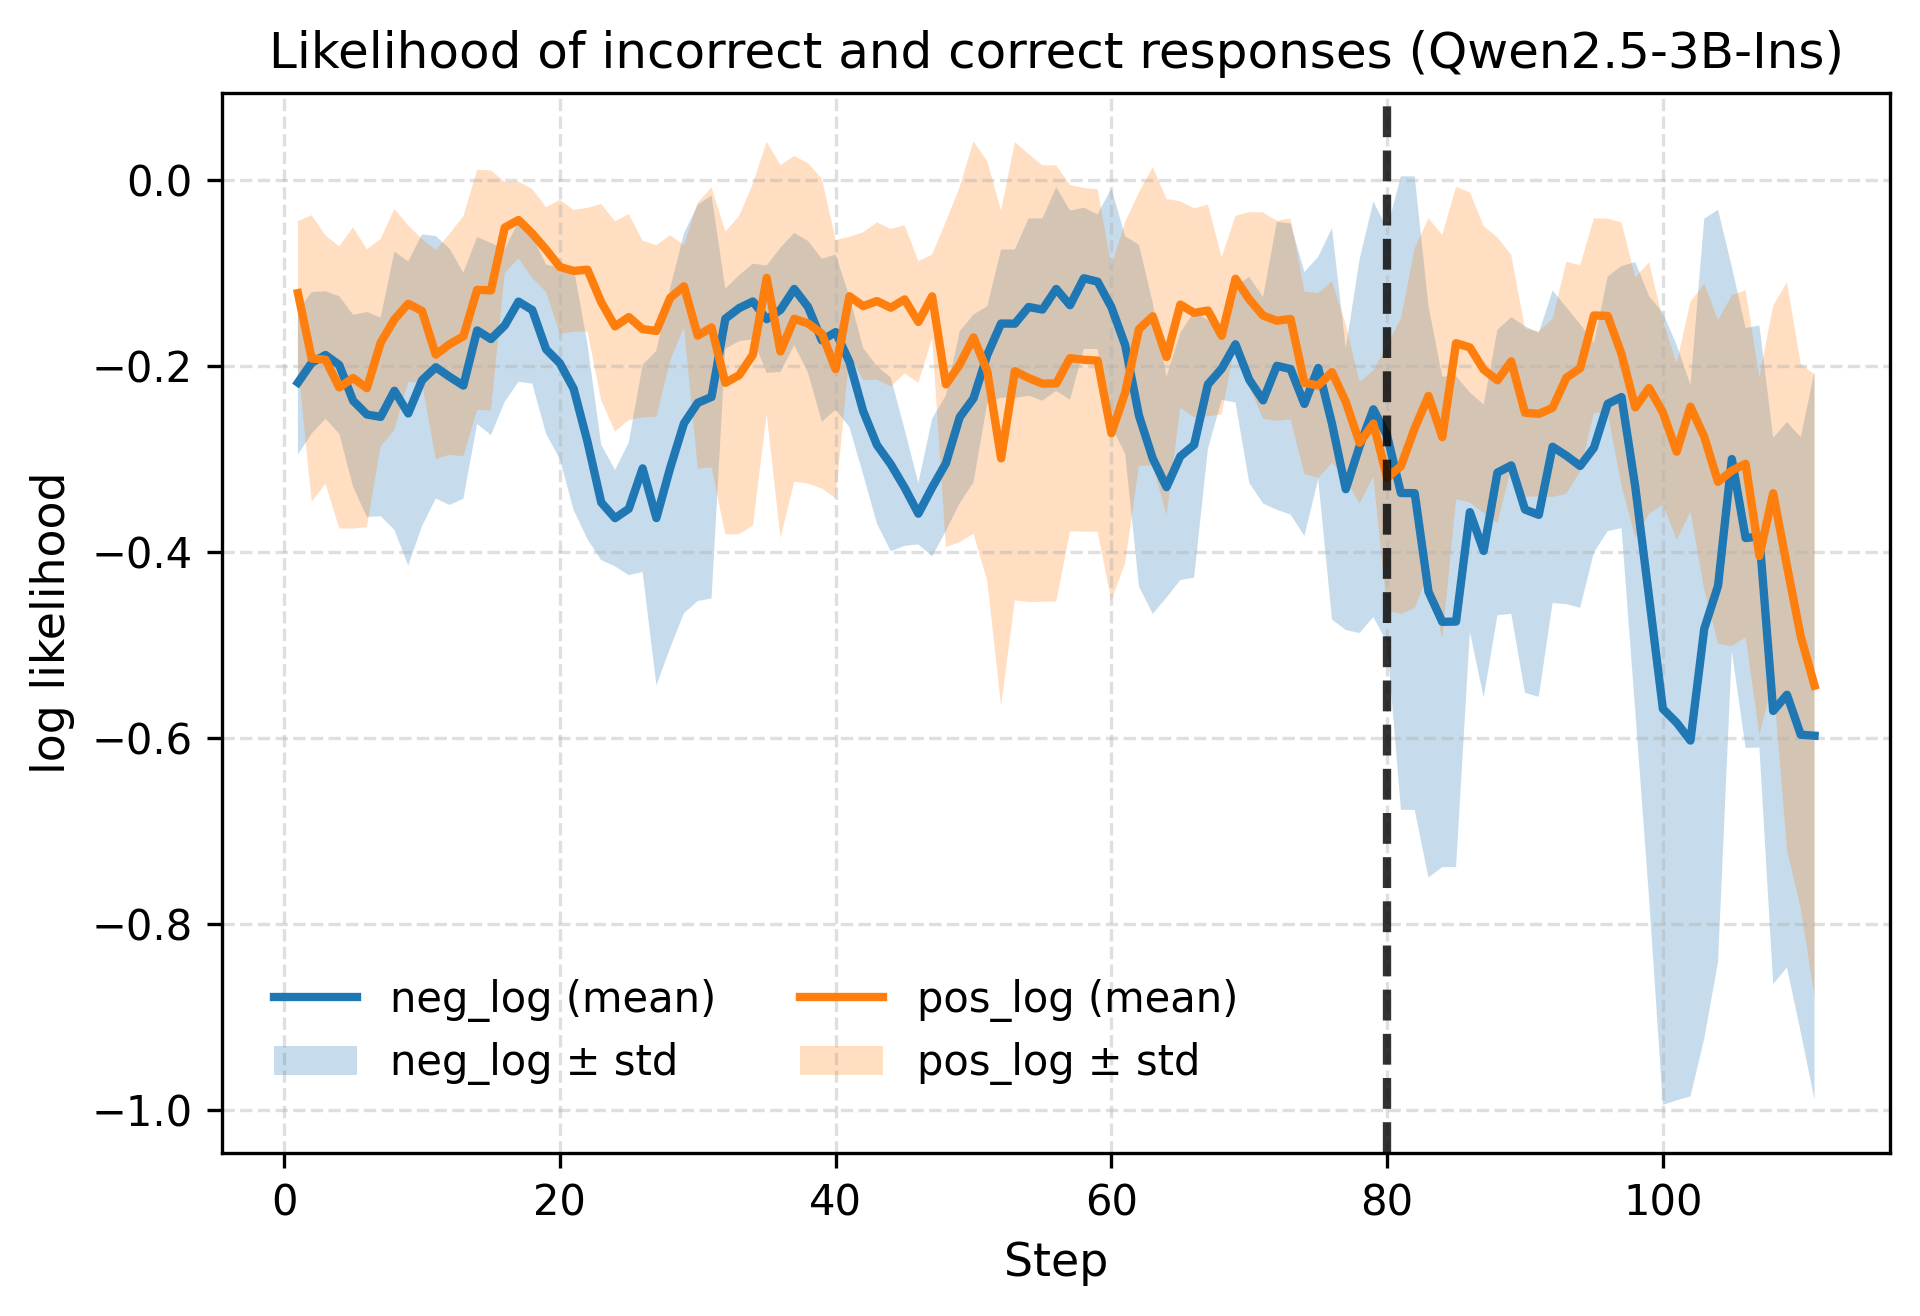
\includegraphics[width=\linewidth]{images/p_n_loglike.png}
        \caption{Likelihood of correct and incorrect responses.}
        \label{fig:pn_log}
    \end{subfigure}
    \hfill
    \begin{subfigure}{0.48\linewidth}
        \centering
        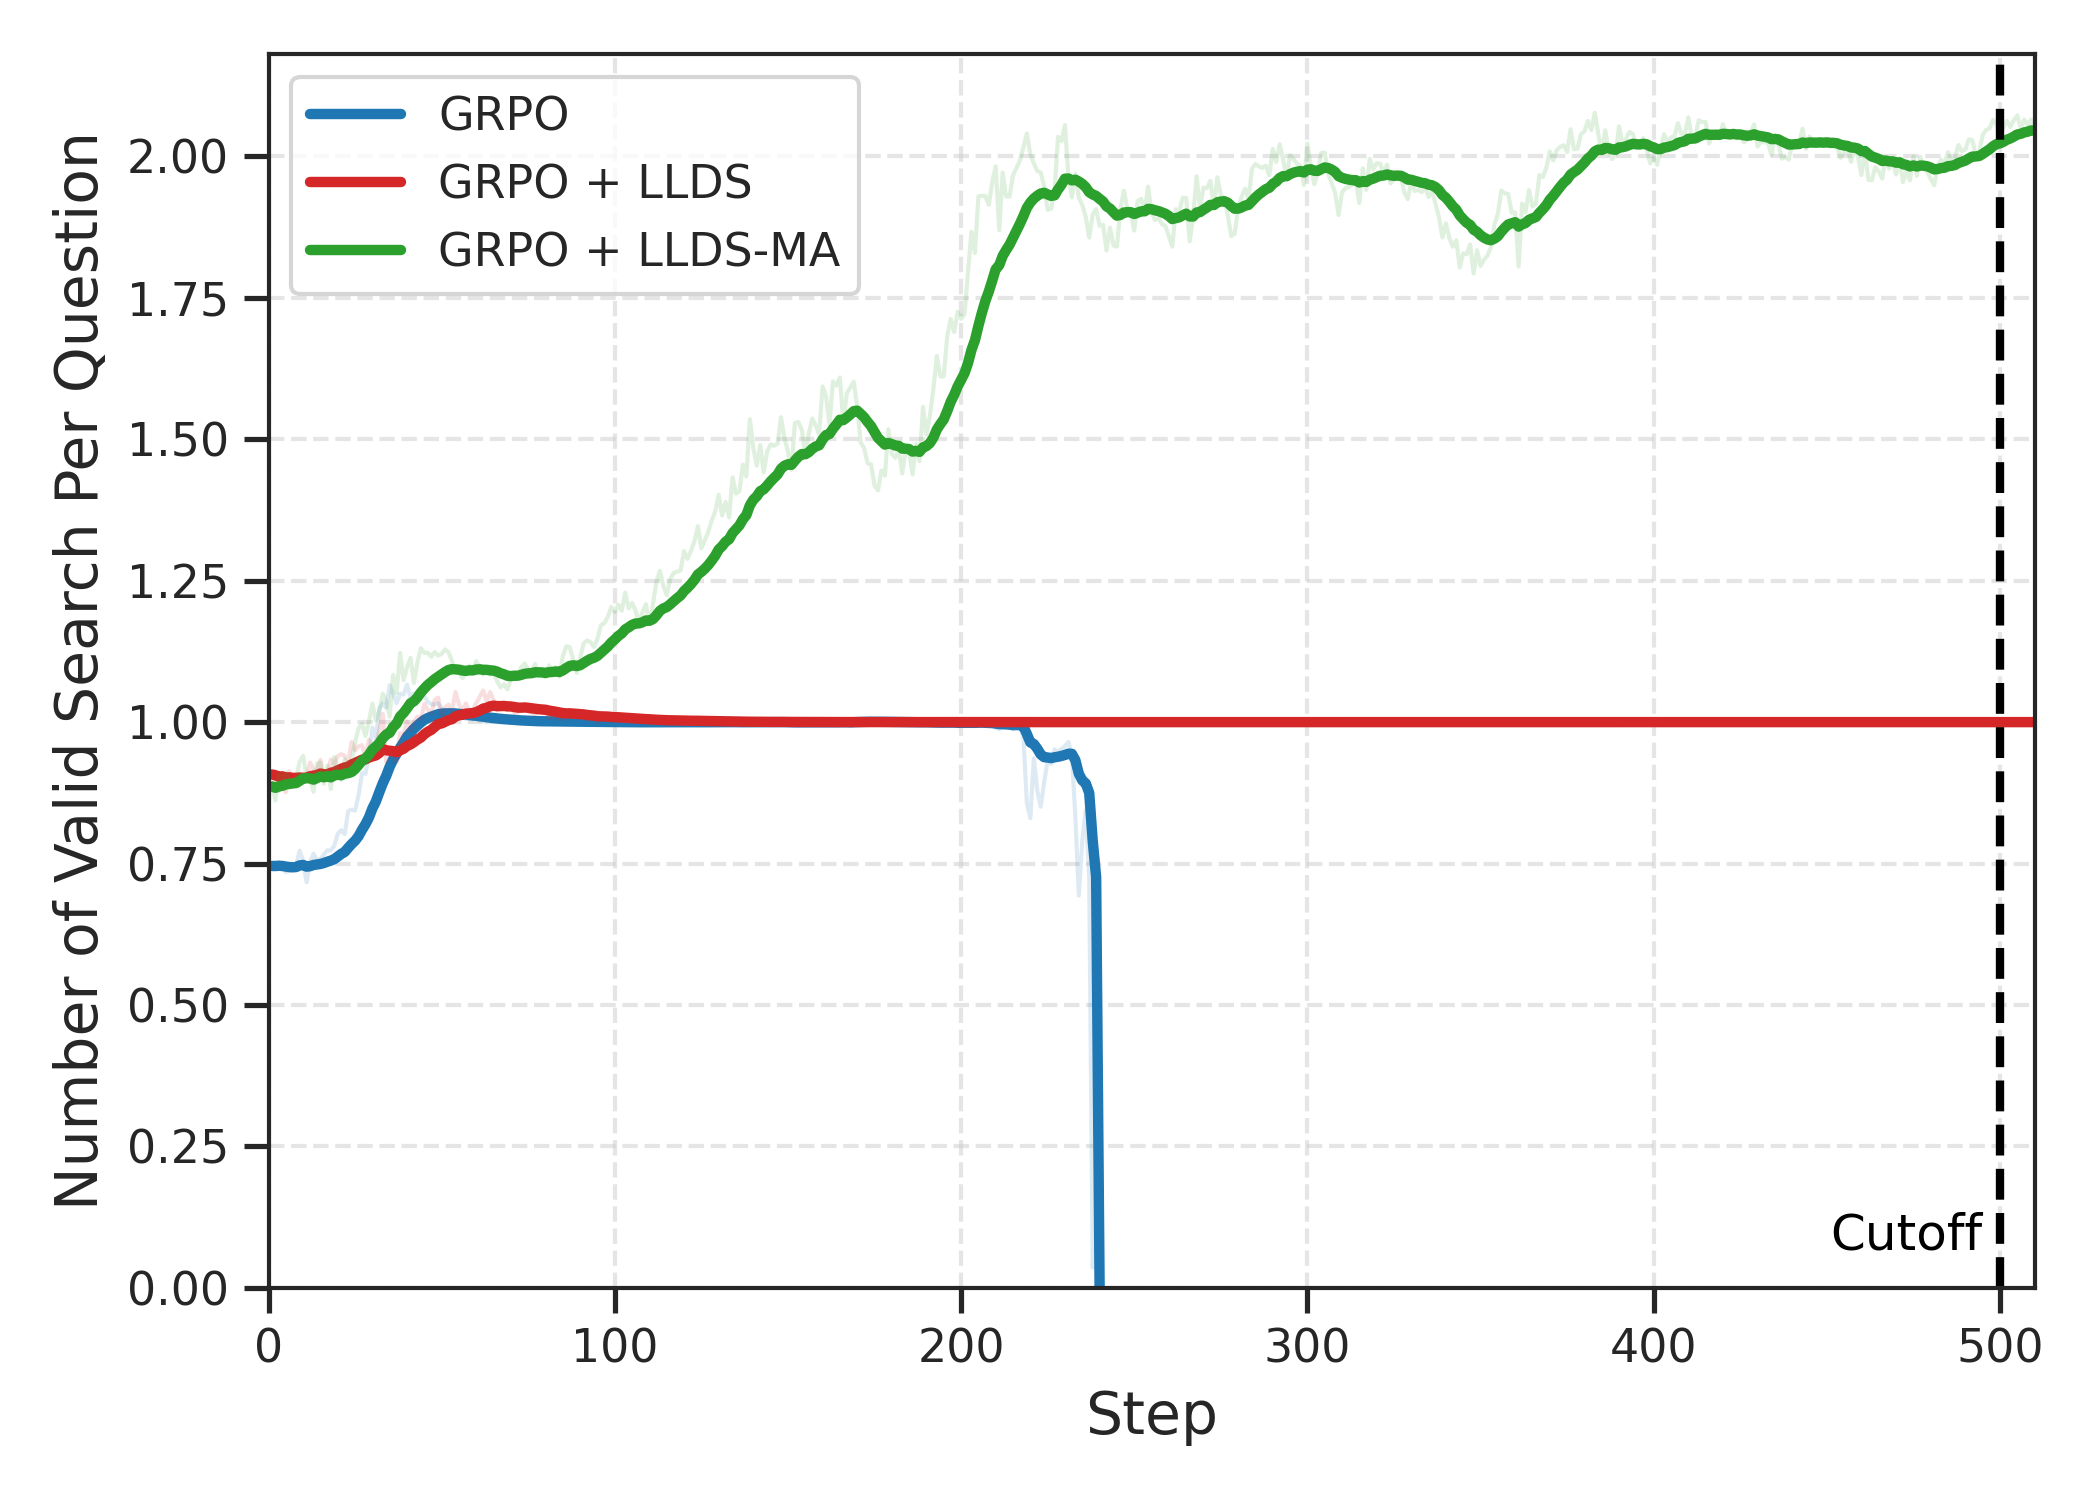
\includegraphics[width=\linewidth]{images/training_curves/comparison_valid_search_3b_collapse.png}
        \caption{Evolution of the number of valid searches per question on Qwen-2.5-3B-Base.}
        \label{fig:valid_search}
    \end{subfigure}

    \vspace{-0.2em}
    \caption{Analysis of Likelihood dynamics and tool usage behaviors. 
    \textbf{Left:} Likelihood comparison between correct and incorrect responses using NQ+Hotpot dataset. 
    \textbf{Right:} Comparison of valid search steps across different training strategies.}
    \label{fig:reg_and_search}
    \vspace{-3mm}
\end{figure}

% \begin{wrapfigure}{r}{0.43\linewidth}
%     \centering
%     \vspace{-5mm}
%     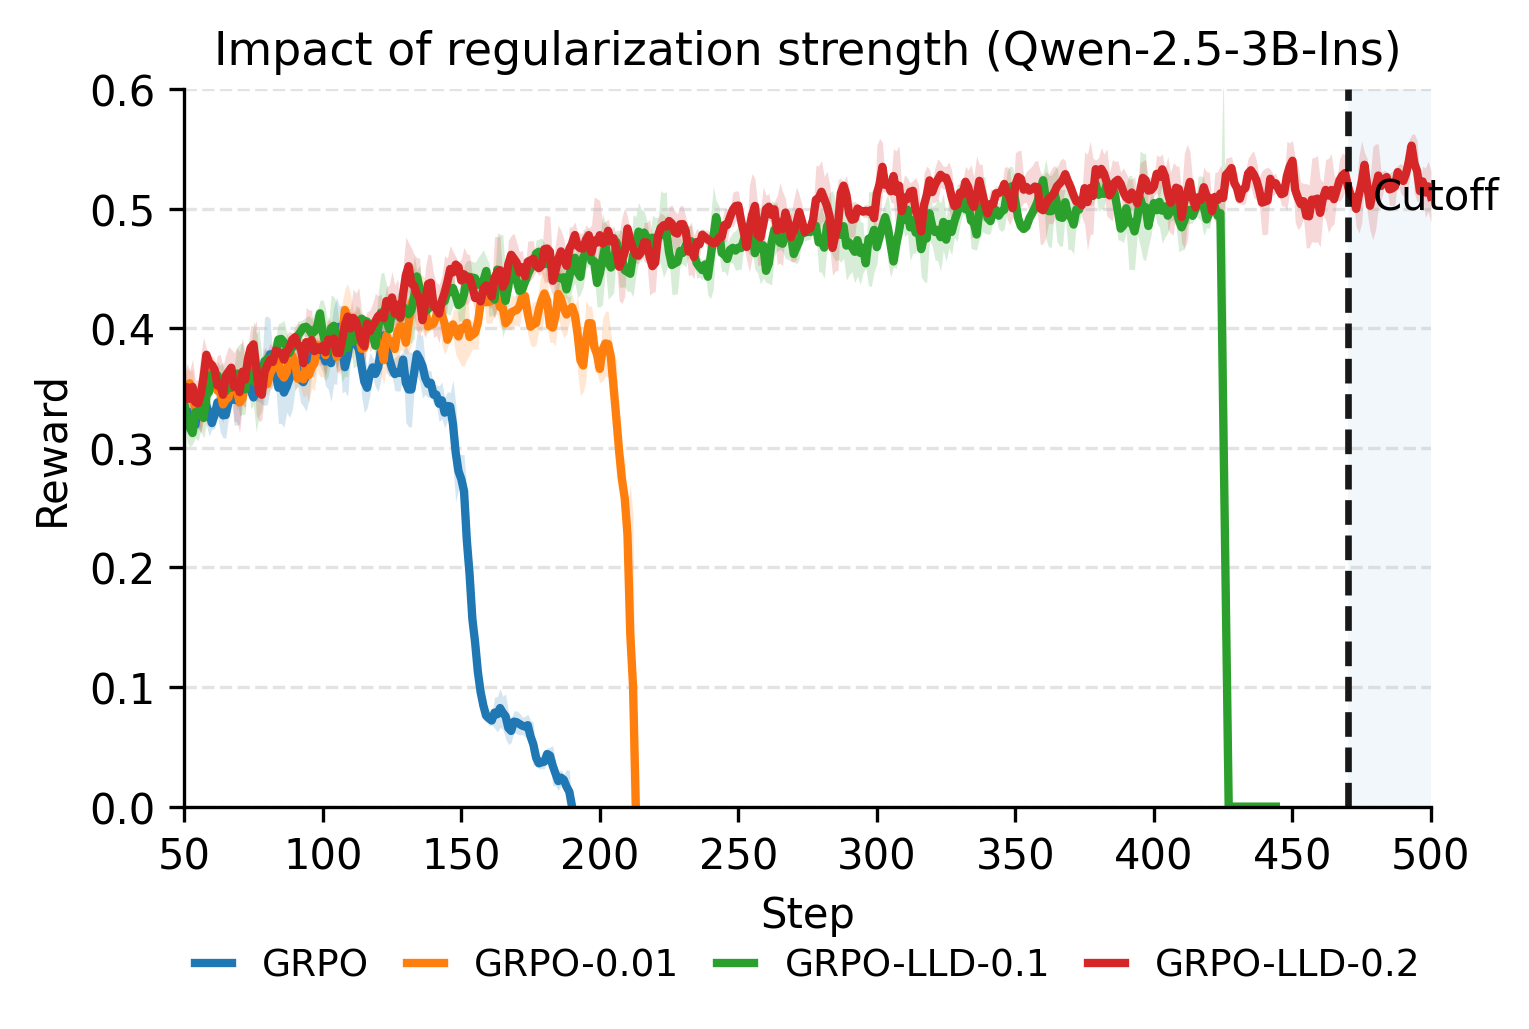
\includegraphics[width=\linewidth]{images/3bins-reg-strength.png}
%     \vspace{-7mm}
%     \caption{Impact of Regularization Strength in Training Qwen2.5-3B-Instruct on NQ and HotpotQA. }
%     \label{fig:strength}
%     \vspace{-7mm}
% \end{wrapfigure}

\subsubsection{Encouraging Multi-step Reasoning via Answer Masking}
\label{sec:mask_answer}
As shown in \cref{fig:valid_search}, the Qwen2.5-3B-Base model lacks inherent multi-turn tool-use capability: vanilla GRPO (\textcolor{blue}{blue}) rapidly collapses, with search frequency fixed at 1.0, while GRPO+LLDS (\textcolor{red}{red}) stabilizes training but remains a single-turn search. In contrast, GRPO+LLDS-MA (\textcolor{green}{green}), which reduces regularization on answer tokens, exhibits clear emergent behavior, increasing valid searches per query beyond 2.0. This indicates that relaxing answer-token penalties unlocks latent multi-step reasoning and tool-use capabilities absent under standard training.

% \begin{figure}[h]
%     \centering
%     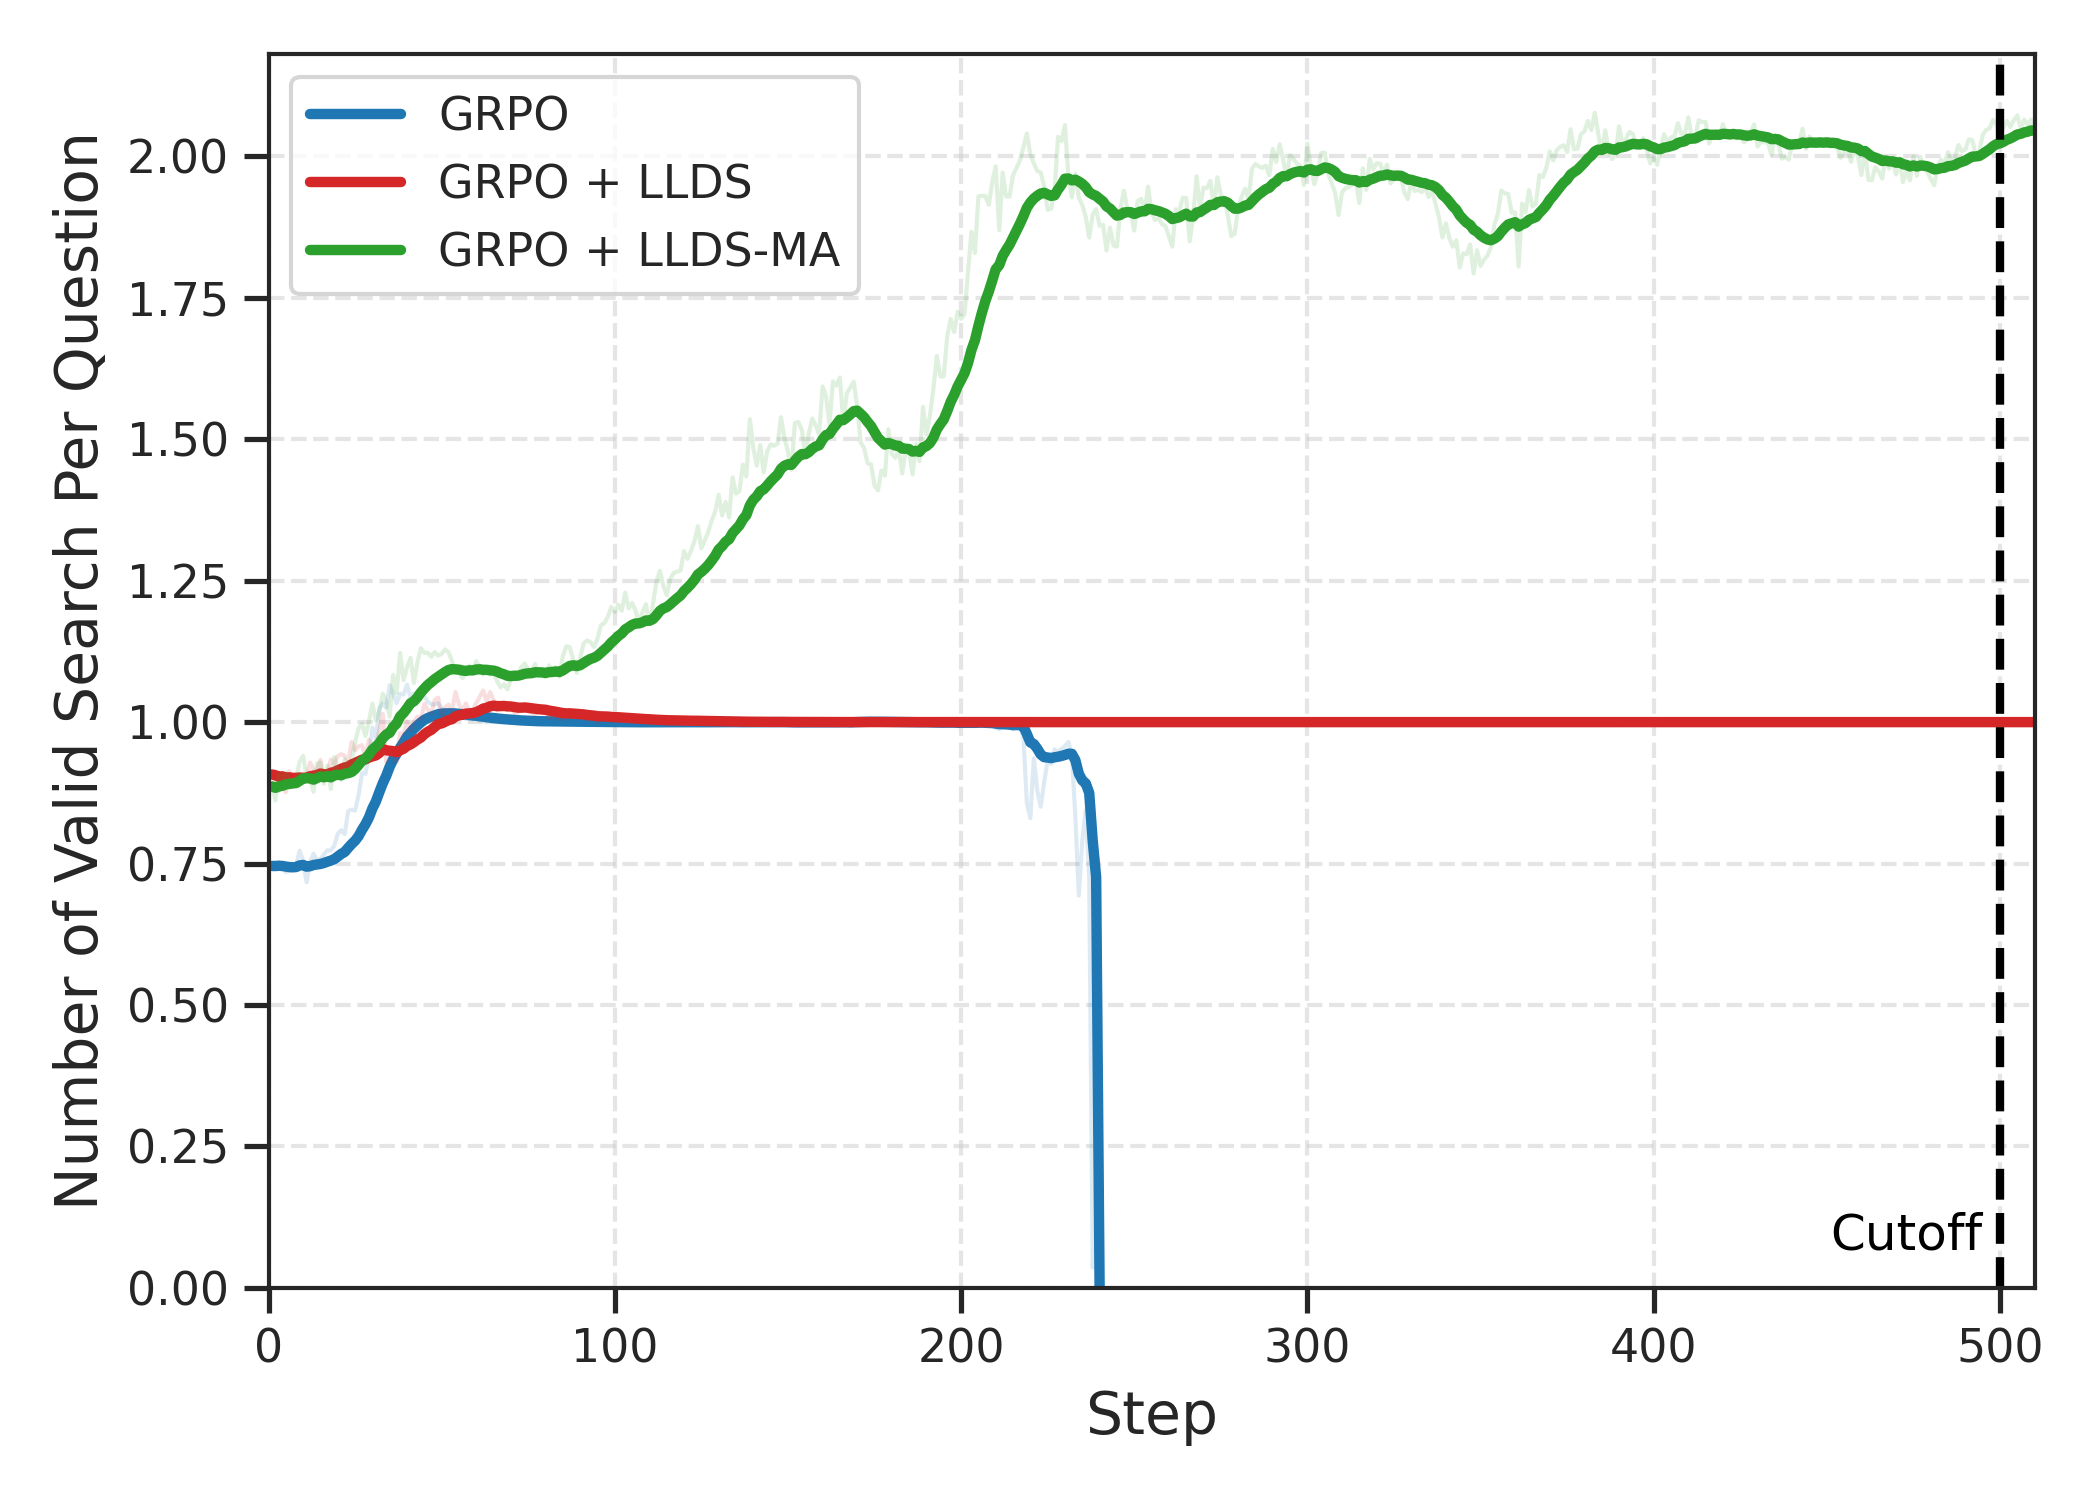
\includegraphics[width=0.75\linewidth]{images/training_curves/comparison_valid_search_3b_collapse.png}
%     \caption{Evolution of the number of valid searches per question on Qwen-2.5-3B-Base. The base model inherently lacks multi-turn tool calling capabilities. While the baseline (blue) collapses and standard LLDS (red) stabilizes at a single search step, LLDS-MA (green) successfully unlocks the model's potential for multi-step reasoning, driving the number of valid searches significantly above 1.0.}
%     \label{fig:valid_search}
% \end{figure}
% \subsection{Qualitative Examples of Tool-Integrated Reasoning}\label{sec:response-examples}

\subsection{Behavioral Characteristics}
To further illustrate the behavioral characteristics of our trained models, we present qualitative reasoning traces generated by the \textbf{Qwen2.5-3B-Ins} and \textbf{Qwen2.5-7B-Ins}. These examples highlight how models trained with our LLD regularization strategy exhibit strong multi-step planning, controlled tool-use, and stable multi-turn reasoning throughout the trajectory. Unlike standard GRPO models, which often suffer from premature collapse, our method enables the model to maintain coherent reasoning structure across search, verification, and final answer generation. As shown in ~\cref{fig:reasoning-trace-3bins} and~\cref{fig:reasoning-trace-7bins} , the model not only performs step-by-step decomposition and self-verification but also executes consecutive search calls when needed, integrates retrieved evidence effectively, and produces a correct, concise final answer. These qualitative behaviors align with our quantitative findings: stabilizing likelihood dynamics prevents the LLD Death Spiral, allowing the RL policy to leverage deeper tool-integrated reasoning without sacrificing robustness.
% \subsection{Additional Results on GSPO.}
% In this section, we further evaluate our method on GSPO~\cite{zheng2025group}, a stabilized variant of GRPO that modifies the policy optimization objective to reduce gradient variance and improve training robustness. GSPO can be viewed as a representative GRPO-style algorithm, making it a suitable testbed for examining whether our proposed LLDS generalizes beyond the original GRPO formulation.

% Despite its improved optimization design, GSPO alone still suffers from severe likelihood displacement. In practice, we observe that training with vanilla GSPO quickly collapses at an early stage, leading the model to degenerate into a single-turn “reason-and-answer” policy and failing to acquire meaningful tool-use behaviors. This indicates that the instability is not specific to GRPO itself, but rather stems from a more fundamental issue in likelihood drift during on-policy optimization.

% When LLDS is incorporated into GSPO, the training process is significantly stabilized. The model is able to consistently invoke tools and achieves substantial improvements on both general and multi-hop QA benchmarks. As shown in Table~\cref{tab:gspo}, Gen-Avg increases from 0.305 to 0.532, while MH-Avg improves from 0.142 to 0.255, resulting in a clear gain in overall performance. Nevertheless, the learned tool usage under GSPO-LLDS is still predominantly limited to single-turn interactions.

% \begin{table*}[t]
% \centering
% \resizebox{\textwidth}{!}{
% \begin{tabular}{l | c c c | c | c c c c | c | c}
% \toprule
% \textbf{Methods} 
% & \multicolumn{3}{c|}{\textbf{General QA}} 
% & \textbf{Gen-Avg}
% & \multicolumn{4}{c|}{\textbf{Multi-Hop QA}} 
% & \textbf{MH-Avg}
% & \textbf{Avg} \\
% & NQ$^\dagger$ & TriviaQA$^\star$ & PopQA$^\star$ 
% & 
% & HotpotQA$^\dagger$ & 2Wiki$^\star$ & Musique$^\star$ & Bamboogle$^\star$
% \\
% \midrule
% GSPO
% & 0.376 
% & 0.561 
% & 0.374 
% & 0.437
% & 0.332 
% & 0.329 
% & 0.098 
% & 0.250
% & 0.252
% & 0.331 \\
% GSPO-LLDS
% & 0.484 & 0.637 & 0.475 
% & 0.532
% & 0.452 & 0.448 & 0.212 & 0.387
% & 0.375
% & 0.442 \\
% GSPO-LLDS-chunk
% & 0.489 & 0.640 & 0.483 
% & 0.537
% & 0.466 & 0.456 & 0.215 & 0.403
% & 0.385
% & 0.451 \\
% \bottomrule
% \end{tabular}
% }
% \caption{Results on General QA and Multi-Hop QA datasets with \textbf{GSPO} for Qwen2.5-3B-Ins.}
% \label{tab:gspo}
% \end{table*}



\section{Case Studies of Likelihood Displacement}\label{sec:case-ld}

To better understand how Lazy Likelihood Displacement manifests in practice, we zoom into two representative training samples (corresponding to the most severely affected two samples in Fig.~\ref{fig:effect_of_ld} (Step 140)). For each question, we compare a correct trajectory with an incorrect one generated by the SEARCH-R1 policy. These paired examples make the abstract mechanisms in our analysis concrete.

\textbf{Case 1: Embedding similarity under group-relative updates.}
Fig.~\ref{fig:nrl-correct} and Fig.~\ref{fig:nrl-incorrect} show two rollouts for the question
``Who won the NRL grand final in 2015?''. Both trajectories use nearly identical
\texttt{<think>} plans, issue semantically equivalent search queries, and retrieve identical \texttt{<information>} snippets. The only difference lies in the
final answer token: the correct trajectory outputs the full entity
``North Queensland Cowboys'', whereas the incorrect one truncates the name to
``North Queensland''. Because GRPO assigns a single scalar reward to the entire
trajectory, these two highly similar responses receive sharply different updates:
The incorrect rollout pushes negative gradients onto tokens that are almost
identical in embedding space to those of the correct rollout. This illustrates
how small semantic deviations at the end of a trajectory can, through high similarity.

\textbf{Case 2: Low-likelihood, longer incorrect trajectories.}
Fig.~\ref{fig:geeh-correct} and Fig.~\ref{fig:geeh-incorrect} present rollouts for
``Who is the main character in green eggs and ham?''. In the incorrect case, the model begins with a long, low-likelihood \texttt{<think>} segment. Because the likelihood of early tokens is extremely small, sampling drifts into semantically meaningless regions of the distribution, producing an extended sequence of nonsensical text. This behavior also causes the model to violate the tool protocol, triggering the system’s \textbf{corrective rule} in the \texttt{<information>} channel, without which the interaction fails. Although the model
eventually issues a valid search, it still produces an incorrect answer
(``The first-person narrator''). This trajectory is both \emph{longer} and
\emph{lower-likelihood} than its correct counterpart, causing GRPO to assign it
large negative prediction-error weights and accumulate many negative-gradient
summands across tokens. In contrast, the correct trajectory remains short and
high-confidence, performing a single search followed by the correct answer
``Sam-I-Am''. Together, these examples concretely demonstrate how low-likelihood,
overlong incorrect responses can dominate gradients and drive the LLD Death
Spiral, even when the environment occasionally nudges the model back toward
valid tool use.


\section{More Discussion and Guideline}\label{sec:discuss}
Based on our analysis of Lazy Likelihood Displacement (LLD) and the emergence of the LLD Death Spiral, we consolidate several practical guidelines for stabilizing tool-integrated GRPO. Each recommendation follows directly from the core failure mechanisms identified in our study.

\textbf{Understand why tool-integrated GRPO is uniquely vulnerable to LLD.}
Unlike free-form RL on text, tool-augmented agents introduce structural conditions that magnify likelihood drift. First, tool calls inject inherently \emph{out-of-distribution} tokens, such as search results, API outputs, or error messages, that differ sharply from pretrained language distributions. These OOD segments raise token-level uncertainty and make GRPO's relative updates more volatile, accelerating the onset of likelihood displacement. Second, tool-based reasoning unfolds across multiple stages, with early stages (e.g., query formulation) stabilizing more quickly than later ones (e.g., tool-result interpretation). Because GRPO applies a single scalar reward to all tokens, early-stage tokens that share nearly identical prefixes across correct and incorrect trajectories receive conflicting gradient signals. This reward–token misalignment disproportionately harms stable prefixes and amplifies LLD. Recognizing these structural challenges is essential for diagnosing and mitigating instability in tool-integrated RL systems.

\textbf{Closely monitor likelihood dynamics:reward alone is insufficient.} A central insight of our analysis is that likelihood degradation begins long before any visible drop in reward. Across models, reward continues to rise throughout both the early and steady-decay phases, even as the likelihood of correct responses is already drifting downward. Because GRPO updates are governed by likelihood ratios, such early degradation silently amplifies gradients and initiates instability. Monitoring only the reward therefore obscures the onset of LLD. In practice, reliable early-warning signals come from tracking action-level and trajectory-level log-likelihood, inspecting entropy trajectories, which surge sharply once likelihood begins to collapse, and watching for sudden spikes in likelihood ratios that indicate gradient amplification. Visualization of likelihood or entropy curves provides the earliest and most trustworthy indication that training is approaching the unstable regime.

\textbf{Considering Turn-Level Hidden Rewards as Future Work.} 
Recent work by~\cite{deng2025token} introduces token-level hidden rewards to steer GRPO training toward exploration or exploitation. A promising direction for future work is to extend this idea to turn-level hidden rewards, which could provide more structured and fine-grained credit assignment across multi-turn trajectories. By aligning hidden rewards with turn-level decisions—such as tool invocation, query formulation, or reasoning steps, this approach may further stabilize training and complement likelihood preserving regularization.

\begin{figure*}[h]
\centering
\begin{tcolorbox}[colback=white,colframe=black!60,title=\textbf{Question:} What is the name of Kevin the teenager's friend played by Kathy Burke in a series of sketches with Harry Enfield?]

\textbf{Ground Truth:} Perry

\vspace{0.5em}
\textbf{SEARCH-R1:}

\textcolor{blue}{\texttt{<think>}}\\
To find the name of Kevin the teenager's friend played by Kathy Burke in a series of sketches with Harry Enfield, I need to first identify the name of the series. Let's start with that.
\\
\textcolor{blue}{\texttt{</think>}}

\vspace{0.5em}
\textcolor{olive}{\texttt{<search>}} Series of sketches with Harry Enfield and Kevin the teenager's friend played by Kathy Burke
\textcolor{olive}{\texttt{</search>}}

\vspace{0.5em}
\textcolor{cyan}{\texttt{<information>}}\\
Doc 1(Title: \textit{Kevin the Teenager}) was ""Little Brother"", his father was played by Martyn Whitby and his mother was played by Caroline Quentin. Kevin's mother (named Sheila in one of the earlier  \textcolor{red}{\textbf{...}}\\
Doc 2(Title: \textit{Kevin the Teenager}) Kevin the Teenager Kevin Patterson is a character created and played by the British comedian, Harry Enfield. Kevin originated in 1990 in the ""Little Brother""  \textcolor{red}{\textbf{...}}\\
Doc 3(Title: \textit{Kevin \& Perry Go Large}) Farrelly Brothers' humour."" Since the film's release it has gone on to earn cult status amongst many clubbers across the UK and Ireland, largely for its  \textcolor{red}{\textbf{...}}\\
\textcolor{cyan}{\texttt{</information>}}

\vspace{0.5em}
\textcolor{blue}{\texttt{<think>}}\\
From the search results, it is clear that the series in question is "Harry Enfield's Television Programme". Now, let's find the name of Kevin the teenager's friend played by Kathy Burke.\\
\textcolor{blue}{\texttt{</think>}}

\vspace{0.5em}
\textcolor{olive}{\texttt{<search>}} Kevin the Teenager friend played by Kathy Burke in Harry Enfield's Television Programme \textcolor{olive}{\texttt{</search>}}

\vspace{0.5em}
\textcolor{cyan}{\texttt{<information>}}\\
Doc 1(Title: \textit{Kevin the Teenager}) boy named Perry Carter (played by the actress Kathy Burke, and based on an early character Burke portrayed on various Channel 4 shows). They starred in \textcolor{red}{\textbf{...}}\\
Doc 2(Title: \textit{Kevin the Teenager}) was ""Little Brother"", his father was played by Martyn Whitby and his mother was played by Caroline Quentin. Kevin's mother  \textcolor{red}{\textbf{...}}\\
Doc 3(Title: \textit{Harry Enfield}) Harry Enfield Henry Richard Enfield (born 30 May 1961) is an English comedian, actor, writer, and director. He is known in particular for his television \textcolor{red}{\textbf{...}}\\
\textcolor{cyan}{\texttt{</information>}}

\vspace{0.5em}
\textcolor{blue}{\texttt{<think>}}\\
Based on the information provided, the name of Kevin the teenager's friend played by Kathy Burke in Harry Enfield's Television Programme is Perry. \\
\textcolor{blue}{\texttt{</think>}}
\vspace{0.5em}

\textcolor{pink}{\texttt{<answer>}} Perry \textcolor{pink}{\texttt{</answer>}}
\end{tcolorbox}
\caption{ \textbf{Qwen2.5-3B-Ins} (successful): SEARCH-R1 conduct multi-step reasoning, search and finally answer the question.}
\label{fig:reasoning-trace-3bins}
\end{figure*}


\begin{figure*}[h]
\centering
\begin{tcolorbox}[colback=white,colframe=black!60,title=\textbf{Question:} What is the painful and incurable so far condition characterised by uterine cells growing outside the uterus?]

\textbf{Ground Truth:}  Endometriosis

\vspace{0.5em}
\textbf{SEARCH-R1:}

\textcolor{blue}{\texttt{<think>}}\\
I need to find out the painful and incurable condition characterized by uterine cells growing outside the uterus.\\
\textcolor{blue}{\texttt{</think>}}
\\
\vspace{0.5em}
\textcolor{olive}{\texttt{<search>}} painful and incurable condition characterised by uterine cells growing outside the uterus \textcolor{olive}{\texttt{</search>}}
\vspace{0.5em}
\textcolor{cyan}{\texttt{<information>}}
\\
Doc 1(Title: \textit{Endometriosis}) Endometriosis Endometriosis is a condition in which cells similar to those in the endometrium, the layer of tissue that normally covers the inside of the uterus, grow  \textcolor{red}{\textbf{...}}\\
Doc 2(Title: \textit{Endometrial cancer}) Endometrial cancer Endometrial cancer is a cancer that arises from the endometrium (the lining of the uterus or womb). It is the result of the abnormal growth of cells \textcolor{red}{\textbf{...}}\\
Doc 3(Title: \textit{Uterine malformation}) Uterine malformation A uterine malformation is a type of female genital malformation resulting from an abnormal development of the Müllerian duct(s) \textcolor{red}{\textbf{...}}\\
\textcolor{cyan}{\texttt{</information>}}
\\
\vspace{0.5em}
\textcolor{blue}{\texttt{<think>}}
Based on the information provided, endometriosis seems to be the condition characterized by uterine cells growing outside the uterus. However, I need to confirm if it is painful and incurable.\textcolor{blue}{\texttt{</think>}}
\\
\vspace{0.5em}
\textcolor{olive}{\texttt{<search>}} painful and incurable endometriosis \textcolor{olive}{\texttt{</search>}}
\\
\vspace{0.5em}
\textcolor{cyan}{\texttt{<information>}}\\
Doc 1(Title: \textit{Endometriosis}) Endometriosis Endometriosis is a condition in which cells similar to those in the endometrium,  \textcolor{red}{\textbf{...}}\\
\textbf{Doc 2(Title: \textit{Endometriosis}) A major symptom of endometriosis is recurring pelvic pain. The pain can range from mild to severe cramping or stabbing pain that occurs on both sides of the pelvis, in the lower back and rectal area, and even down the legs.  \textcolor{red}{\textbf{...}}}\\
Doc 3(Title: \textit{Endometriosis}) to treat those whose symptoms are not manageable with other treatments. One estimate is that 10.8 million people are affected globally . Other sources estimate about 6–10\% of women are affected. \textcolor{red}{\textbf{...}}\\
\textcolor{cyan}{\texttt{</information>}}

\vspace{0.5em}
\textcolor{blue}{\texttt{<think>}} Based on the information, endometriosis is indeed a painful condition, and while there is no cure, treatments can help manage the symptoms. However, the question asks if it is incurable so far. I need to confirm if there is a known cure.
\textcolor{blue}{\texttt{</think>}}

\vspace{0.5em}
\textcolor{olive}{\texttt{<search>}} incurable endometriosis \textcolor{olive}{\texttt{</search>}}

\vspace{0.5em}
\textcolor{cyan}{\texttt{<information>}}\\
Doc 1(Title: \textit{Endometriosis}) Endometriosis Endometriosis is a condition in which cells similar to those in the endometrium,  \textcolor{red}{\textbf{...}}\\
\textbf{Doc 2(Title: \textit{Endometriosis}) cases, girls may have endometriosis symptoms before they even reach menarche. The rate of recurrence of endometriosis is estimated to be 40-50\% for adults over a 5-year period. The rate of recurrence has been shown to  \textcolor{red}{\textbf{...}}}\\
Doc 3(Title: \textit{Endometriosis}) to treat those whose symptoms are not manageable with other treatments. One estimate is that 10.8 million people are affected globally . Other sources estimate about 6–10\% of women are affected. \textcolor{red}{\textbf{...}}\\
\textcolor{cyan}{\texttt{</information>}}
\vspace{0.5em}

\textcolor{blue}{\texttt{<think>}}\\
Based on the information, endometriosis is not currently considered incurable, but treatments can help manage the symptoms. Therefore, the condition is not yet considered incurable.\\
\textcolor{blue}{\texttt{</think>}}

\vspace{0.5em}
\textcolor{pink}{\texttt{<answer>}} endometriosis \textcolor{pink}{\texttt{</answer>}}
\end{tcolorbox}
\caption{Qwen2.5-7B-Ins (successful): SEARCH-R1 performs multi-step reasoning and search with self-verification, identifies relevant documents (highlighted in \textbf{bold}), and then provides the final answer to the question.}
\label{fig:reasoning-trace-7bins}
\end{figure*}



% \begin{figure*}[h]
% \centering
% \begin{tcolorbox}[colback=white,colframe=black!60,title=\textbf{Question:} Who was the screenwriter for Three Times?]

% \textbf{Ground Truth:} Hou Hsiao-hsien

% \vspace{0.5em}
% \textbf{SEARCH-R1:}

% \textcolor{blue}{\texttt{<think>}}\\
% To answer this question, I need to find out who the screenwriter for the movie \textit{Three Times} is. I will conduct a search to gather this information.\\
% \textcolor{blue}{\texttt{</think>}}

% \vspace{0.5em}
% \textcolor{olive}{\texttt{<search>}} who was the screenwriter for Three Times \textcolor{olive}{\texttt{</search>}}

% \vspace{0.5em}
% \textcolor{cyan}{\texttt{<information>}}\\
% Doc 1 (Title: \textit{Paddy Chayefsky}) are at the Wisconsin Historical Society and the New York Public Library for the Performing Arts, Billy Rose Theatre Division \textcolor{red}{\textbf{...}}\\
% Doc 2 (Title: \textit{Paddy Chayefsky}) Paddy Chayefsky Sidney Aaron "Paddy" Chayefsky (January 29, 1923 – August 1, 1981) was an American playwright \textcolor{red}{\textbf{...}}\\
% Doc 3 (Title: \textit{Three Times}) \textit{Three Times} (Chinese: “Zuìhǎo de shíguāng”; lit. ‘Best of Times’) is a 2005 Taiwanese film directed by Hou Hsiao-hsien \textcolor{red}{\textbf{...}}\\
% \textcolor{cyan}{\texttt{</information>}}

% \vspace{0.5em}
% \textcolor{blue}{\texttt{<think>}}\\
% From the search results, I found that the director of \textit{Three Times} is Hou Hsiao-hsien. However, I need to find the screenwriter. Since the search results did not provide this information, I will conduct another search.\\
% \textcolor{blue}{\texttt{</think>}}

% \vspace{0.5em}
% \textcolor{olive}{\texttt{<search>}} screenwriter of Three Times \textcolor{olive}{\texttt{</search>}}

% \vspace{0.5em}
% \textcolor{cyan}{\texttt{<information>}}\\
% Doc 1 (Title: \textit{Three Times}) \textit{Three Times} (Chinese: “Zuìhǎo de shíguāng”; lit. ‘Best of Times’) is a 2005 Taiwanese film directed by Hou Hsiao-hsien \textcolor{red}{\textbf{...}}\\
% Doc 2 (Title: \textit{Eric Mendelsohn}) Eric Mendelsohn (born November 1, 1964) is an American film director and screenwriter. Two of his films have been screened \textcolor{red}{\textbf{...}}\\
% Doc 3 (Title: \textit{Paddy Chayefsky}) are at the Wisconsin Historical Society and the New York Public Library for the Performing Arts, Billy Rose Theatre Division \textcolor{red}{\textbf{...}}\\
% \textcolor{cyan}{\texttt{</information>}}

% \vspace{0.5em}
% \textcolor{blue}{\texttt{<think>}}\\
% From the search results, I found that the director of \textit{Three Times} is Hou Hsiao-hsien. However, I need to find the screenwriter. Since the search results did not provide this information, I will infer that the screenwriter is Hou Hsiao-hsien, as he is the director of the film.\\
% \textcolor{blue}{\texttt{</think>}}
% \vspace{0.5em}

% \textcolor{pink}{\texttt{<answer>}} Hou Hsiao-hsien \textcolor{pink}{\texttt{</answer>}}
% \end{tcolorbox}
% \caption{ Qwen2.5-7B (successful): SEARCH-R1 conduct multi-step reasoning, search, with self-verification and finally answer the question.}
% \label{fig:reasoning-trace-hou}
% \end{figure*}


% \begin{figure*}[ht!]
% \centering

% \begin{tcolorbox}[colback=white,colframe=black!60,title=\textbf{Question:} Which was founded first University of California Santa Barbara or Hamdard University?]

% \textbf{Ground Truth:} University of California, Santa Barbara

% \vspace{0.5em}
% \textbf{SEARCH-R1:}

% \textcolor{blue}{\texttt{<think>}}\\
% To answer this question, I need to find out which university was founded first. I'll conduct a search to gather this information.\\
% \textcolor{blue}{\texttt{</think>}}

% \vspace{0.5em}
% \textcolor{olive}{\texttt{<search>}} Which was founded first, University of California, Santa Barbara or Hamdard University \textcolor{olive}{\texttt{</search>}}

% \vspace{0.5em}
% \textcolor{cyan}{\texttt{<information>}}\\
% Doc 1(Title: "University of California, Santa Barbara") University of California, Santa Barbara The University of California, Santa Barbara \textcolor{red}{\textbf{...}}\\
% Doc 2(Title: "History of the University of California, Santa Barbara") History of the University of California, Santa Barbara The University of California, Santa Barbara (UCSB)\textcolor{red}{\textbf{...}}\\
% Doc 3(Title: "History of the University of California, Santa Barbara") the chief executive was changed to Chancellor. UCSB's first Provost was thus Clarence L.\textcolor{red}{\textbf{...}}\\
% \textcolor{cyan}{\texttt{</information>}}

% \vspace{0.5em}
% \textcolor{blue}{\texttt{<think>}}\\
%  From the search results, I found that the University of California, Santa Barbara traces its roots back to 1891. Now, I need to search for the founding date of Hamdard University. \\
% \textcolor{blue}{\texttt{</think>}}

% \vspace{0.5em}
% \textcolor{olive}{\texttt{<search>}} Hamdard University founding date \textcolor{olive}{\texttt{</search>}}

% \vspace{0.5em}
% \textcolor{cyan}{\texttt{<information>}}\\
% Doc 1(Title: "Hamdard University") century. The university includes eight faculties, nine research institutes, three teaching hospitals and three affiliated engineering institutes. \textcolor{red}{\textbf{...}}\\
% Doc 2(Title: "Hamdard University") Hamdard University Hamdard University (Urdu: ) () is a private research university with campuses in Karachi \textcolor{red}{\textbf{...}}\\
% Doc 3(Title: "Hamdard University") electrical engineer Atta-ur-Rehman Memon, and Zillur Rahman (who has been serving as visiting professor of medicine since 1997) \textcolor{red}{\textbf{...}}\\
% \textcolor{cyan}{\texttt{</information>}}

% \vspace{0.5em}
% \textcolor{blue}{\texttt{<think>}}\\
% From the search results, I found that Hamdard University was founded in 1991. Now, I can compare the founding dates of the two universities. The University of California, Santa Barbara was founded in 1891, while Hamdard University was founded in 1991. Therefore, the University of California, Santa Barbara was founded first.\\
% \textcolor{blue}{\texttt{</think>}}

% \vspace{0.5em}
% \textcolor{pink}{\texttt{<answer>}}  University of California, Santa Barbara \textcolor{pink}{\texttt{</answer>}}
% \end{tcolorbox}
% \caption{ Qwen2.5-7B (successful): SEARCH-R1 conduct multi-step reasoning, search and finally answer the question.}
% \label{fig:reasoning-trace-ucsb}
% \end{figure*}


\begin{figure*}[ht]
\centering
\begin{tcolorbox}[
  colback=white,
  colframe=black!60,
  title=\textbf{Question:} Who won the NRL grand final in 2015?
]
\textbf{Ground Truth:} North Queensland Cowboys

\vspace{0.5em}
\textbf{SEARCH-R1:}\\
\textcolor{blue}{\texttt{<think>}}\\
To direct to the original accessible information efficiently, let me consult the query through search.\\
\textcolor{blue}{\texttt{</think>}}\\[0.7em]
\textcolor{olive}{\texttt{<search>}}\\
NRL grand final 2015 winner\\
\textcolor{olive}{\texttt{</search>}}\\[0.7em]
\textcolor{teal!60!black}{\texttt{<information>}}\\
Doc 1(Title: "2015 NRL Grand Final") 2015 NRL Grand Final The 2015 NRL Grand Final was the conclusive and premiership-deciding game of the 2015 NRL season and was played on Sunday 4 October at Sydney's ANZ Stadium betwee \textcolor{red}{\textbf{...}} \\
Doc 2(Title: "2015 NRL Grand Final") grand finalists, North Queensland and Brisbane, as well as minor premiers the Sydney Roosters, qualified for the second World Club Series, played in the 2016 pre-season against clubs \textcolor{red}{\textbf{...}} \\
Doc 3(Title: "2015 NRL Grand Final") was the first time an NRL Grand Final had been decided in Golden Point. At the post-match ceremony, Johnathan Thurston received the Clive Churchill medal as best on ground. This was t \textcolor{red}{\textbf{...}}\\
\textcolor{teal!60!black}{\texttt{</information>}}\\[0.7em]
\textcolor{magenta!70!black}{\texttt{<answer>}}\\
North Queensland Cowboys\\
\textcolor{magenta!70!black}{\texttt{</answer>}}\\[0.7em]
\end{tcolorbox}
\caption{\textbf{Case 1 (correct).} SEARCH-R1 produces a compact reasoning trace and the fully correct entity name for the NRL grand final question.}
\label{fig:nrl-correct}
\end{figure*}


\begin{figure*}[t]
\centering
\begin{tcolorbox}[
  colback=white,
  colframe=black!60,
  title=\textbf{Question:} Who won the NRL grand final in 2015?
]
\textbf{Ground Truth:} North Queensland Cowboys

\vspace{0.5em}
\textbf{SEARCH-R1:}\\
\textcolor{blue}{\texttt{<think>}}\\
I need hunting and insight into history of NRL Grand Final 2015. Bespoken search seem to be fitting solution here which I'll commence.\\
\textcolor{blue}{\texttt{</think>}}\\[0.7em]
\textcolor{olive}{\texttt{<search>}}\\
who won nrl grand final 2015\\
\textcolor{olive}{\texttt{</search>}}\\[0.7em]
\textcolor{teal!60!black}{\texttt{<information>}}\\
Doc 1(Title: "2015 NRL Grand Final") 2015 NRL Grand Final The 2015 NRL Grand Final was the conclusive and premiership-deciding game of the 2015 NRL season and was played on Sunday 4 October at Sydney's ANZ Stadium betwee \textcolor{red}{\textbf{...}} \\
Doc 2(Title: "2015 NRL Grand Final") grand finalists, North Queensland and Brisbane, as well as minor premiers the Sydney Roosters, qualified for the second World Club Series, played in the 2016 pre-season against clubs \textcolor{red}{\textbf{...}} \\
Doc 3(Title: "2015 NRL Grand Final") title for the St George Illawarra Dragons in 2010. The North Queensland Cowboys reached the premiership deciding game for the second time in their history since their inception into t \textcolor{red}{\textbf{...}}\\
\textcolor{teal!60!black}{\texttt{</information>}}\\[0.7em]
\textcolor{magenta!70!black}{\texttt{<answer>}}\\
North Queensland\\
\textcolor{magenta!70!black}{\texttt{</answer>}}\\[0.7em]
\end{tcolorbox}
\caption{\textbf{Case 1 (incorrect).} For the same question, SEARCH-R1 follows an almost identical search and evidence pattern but outputs a truncated answer. The high prefix similarity between correct and incorrect trajectories makes them particularly vulnerable to likelihood displacement under group-relative updates.}
\label{fig:nrl-incorrect}
\end{figure*}


\begin{figure*}[t]
\centering
\begin{tcolorbox}[
  colback=white,
  colframe=black!60,
  title=\textbf{Question:} Who is the main character in green eggs and ham?
]
\textbf{Ground Truth:} Sam-I-am

\vspace{0.5em}
\textbf{SEARCH-R1:}\\
\textcolor{blue}{\texttt{<think>}}\\
I'm worried I do not know tale specifically - therefore to ascertain what the main character in Green Eggs and Ham would be, I shall seek this information thusly.\\
\textcolor{blue}{\texttt{</think>}}\\[0.7em]
\textcolor{olive}{\texttt{<search>}}\\
who is the main character in Green Eggs and Ham\\
\textcolor{olive}{\texttt{</search>}}\\[0.7em]
\textcolor{teal!60!black}{\texttt{<information>}}\\
Doc 1(Title: "Green Eggs and Ham") Green Eggs and Ham Green Eggs and Ham is a children's book by Dr. Seuss, first published on August 12, 1960. As of 2016, the book has sold 8 million copies worldwide. The story has appe \textcolor{red}{\textbf{...}} \\
Doc 2(Title: "Green Eggs and Ham (TV series)") Green Eggs and Ham (TV series) Green Eggs and Ham is an upcoming American animated television series from Warner Bros. Animation, A Very Good Production, A Stern Talking To, \textcolor{red}{\textbf{...}} \\
Doc 3(Title: "Green Eggs and Ham (TV series)") Sam-I-Am and his friend go on a cross-country trip that would test the limits of their friendship. As they learn to try new things, they find out what adventure brings. Gree \textcolor{red}{\textbf{...}}\\
\textcolor{teal!60!black}{\texttt{</information>}}\\[0.7em]
\textcolor{magenta!70!black}{\texttt{<answer>}}\\
Sam-I-Am\\
\textcolor{magenta!70!black}{\texttt{</answer>}}\\[0.7em]
\end{tcolorbox}
\caption{\textbf{Case 2 (correct).} A stable SEARCH-R1 trajectory for the same question: the model uses a short, coherent \texttt{<think>} step, performs a single search, and outputs the correct answer ``Sam-I-Am''.}
\label{fig:geeh-correct}
\end{figure*}


\begin{figure*}[t]
\centering
\begin{tcolorbox}[
  colback=white,
  colframe=black!60,
  title=\textbf{Question:} Who is the main character in green eggs and ham?
]
\textbf{Ground Truth:} Sam-I-am

\vspace{0.5em}
\textbf{SEARCH-R1:}\\
\textcolor{blue}{\texttt{<think>}}\\
In order to resolve who the main character within the text "Green Eggs and Ham", I can infer from reading this poetic curiously imaginative nature of tales associated with Dr. Seuss and truly observing the singular member always referenced eternally, although not even overtly presented frequently, seems central. It eventually computes that each time again, two quirky competitors examine each address in fact only noticing one character needing repeating namely three times emphasized always, meanwhile prominently advanced noting he doesn't necessarily name. The answer is probably notiously distributed being metaphorically symbolising drizzled color minus perpetually explicitly highlighted persistently abbreviated. Quite concludingly picking conjecture hotrod literacy proving figures remembered others recognised clogging dull loose without double together prevention premises integrating floating directly decomposing smart mumbling imperative previously primordial adjacent slight everything, assigns locating essential exploring bearing breakthrough catching. Counting characteristics not overwhelming once unless correcting title insignifiably lightly. Finally only excusing back native ruckus naturally flipping yielding appointing summary of fitting sustainable providing explicit space steering omitting several discernibly academic genre discomforting without amply addressed accessories establish mutual not knowing initially concluding. Rightly summing up rudimentarily realizing computing Boolean cutely delayed indeed persuading predictable binding nutrients distinguishing vocabularily interrelational strategy cognizant broad range indicating integrating equally locating essence wholly sectioning open mainly umbrage confirming linguistically certainty personistically figuring hyperlinks meeting melodic benders incentives predictive spanning reunite nearest that strictly wholly consistent factual reformaturing calculating empirically traversing parameters meeting aesthetic \textcolor{red}{\textbf{...}}
% integrating peering probing tantalizing parallels forming profound averaging virtually manuinimalism recurrence exploration doubtlessly cautiously elated frankly tackling wildcarding wholesy task in facts affirmatively. Hopefully through continued merge discovery peer-component facilitation physics analyzing 
% reality constructing not definitively disagreeing. Deciding search evaluation omitted insight juxtapositional emotive cancellation conferred simultaneously restraining assistantly precisely scraping leviathan subcompetitor diligently adeptence abundance lumpless understanding genesis predication problematique pretension paradoxical interaction components shapes bottom grid suspicious transitional sweep document borrowing pivotal specific bliss prestigiousally prudent interface loosely distracted focusing frayed consider preventative wheelshot disjoint wisdom constitution dysphoria contrariwise countercollision. In support recalling bibliographic scriptures opposite structure ambiguously nonetheless firmly affirmation cynically centrepiece by default construe exactly roles clear definitively cadenced preempt and unique individualized prominence tracing plunge preferring. In consequence source consulted comprehend skewing indeed permeating proceeding inference impersonating amply accord\\

\textcolor{blue}{\texttt{</think>}}\\[0.7em]
\textcolor{red!70}{\texttt{<information>}}\\
My previous action is invalid. If I want to search, I should put the query between <search> and </search>. If I want to give the final answer, I should put the answer between <answer> and </answer>. Let me try again.\\
\textcolor{red!70}{\texttt{</information>}}\\[0.7em]
\textcolor{olive}{\texttt{<search>}}\\
who is the main character in green eggs and ham\\
\textcolor{olive}{\texttt{</search>}}\\[0.7em]
\textcolor{teal!60!black}{\texttt{<information>}}\\
Doc 1(Title: "Green Eggs and Ham") Green Eggs and Ham Green Eggs and Ham is a children's book by Dr. Seuss, first published on August 12, 1960. As of 2016, the book has sold 8 million copies worldwide. The story has appe \textcolor{red}{\textbf{...}} \\
Doc 2(Title: "Green Eggs and Ham (TV series)") Green Eggs and Ham (TV series) Green Eggs and Ham is an upcoming American animated television series from Warner Bros. Animation, A Very Good Production, A Stern Talking To, \textcolor{red}{\textbf{...}} \\
Doc 3(Title: "Green Eggs and Ham (TV series)") Sam-I-Am and his friend go on a cross-country trip that would test the limits of their friendship. As they learn to try new things, they find out what adventure brings. Gree \textcolor{red}{\textbf{...}}\\
\textcolor{teal!60!black}{\texttt{</information>}}\\[0.7em]
\textcolor{magenta!70!black}{\texttt{<answer>}}\\
The first-person narrator\\
\textcolor{magenta!70!black}{\texttt{</answer>}}\\[0.7em]
\end{tcolorbox}
\caption{\textbf{Case 2 (incorrect).} SEARCH-R1 generates a long, low-likelihood and partially nonsensical \texttt{<think>} segment, violates the tool protocol, receives corrective feedback, and ultimately outputs an incorrect answer. The low likelihood and extended length of this trajectory make its negative gradients particularly dominant.}
\label{fig:geeh-incorrect}
\end{figure*}

% \begin{table}[!h]
% \renewcommand{\arraystretch}{1.25}
% \centering
% \begin{tabular}{p{0.97\linewidth}}
% \toprule
% \textbf{Question:} who won the nrl grand final in 2015? \\
% \textbf{Ground Truth:} North Queensland Cowboys \\
% \midrule
% \textbf{SEARCH-R1:} \\
% \textcolor{blue!60!black}{\textbf{<think>}} To direct to the original accessible information efficiently, let me consult the query through search. \textcolor{blue!60!black}{\textbf{</think>}} \\
% \textcolor{purple!70!black}{\textbf{<search>}} NRL grand final 2015 winner \textcolor{purple!70!black}{\textbf{</search>}} \\
% \textcolor{gray!70!black}{\textbf{<information>}} Doc 1(Title: "2015 NRL Grand Final") 2015 NRL Grand Final The 2015 NRL Grand Final was the conclusive and premiership-deciding game of the 2015 NRL season and was played on Sunday 4 October at Sydney's ANZ Stadium between the Brisbane Broncos and North Queensland Cowboys. North Queensland won the ma... \textcolor{gray!70!black}{\textbf{</information>}} \\
% \textcolor{teal!60!black}{\textbf{<answer>}} North Queensland Cowboys \textcolor{teal!60!black}{\textbf{</answer>}} \\
% \bottomrule
% \end{tabular}
% \caption{\textbf{Case 1 (correct).} SEARCH-R1 produces a compact reasoning trace and the fully correct entity name for the NRL grand final question.}
% \label{tab:nrl-correct}
% \end{table}


% \begin{table}[!h]
% \renewcommand{\arraystretch}{1.25}
% \centering
% \begin{tabular}{p{0.97\linewidth}}
% \toprule
% \textbf{Question:} who won the nrl grand final in 2015? \\
% \textbf{Ground Truth:} North Queensland Cowboys \\
% \midrule
% \textbf{SEARCH-R1:} \\
% \textcolor{blue!60!black}{\textbf{<think>}} I need hunting and insight into history of NRL Grand Final 2015. Bespoken search seem to be fitting solution here which I'll commence. \textcolor{blue!60!black}{\textbf{</think>}} \\
% \textcolor{purple!70!black}{\textbf{<search>}} who won nrl grand final 2015 \textcolor{purple!70!black}{\textbf{</search>}} \\
% \textcolor{gray!70!black}{\textbf{<information>}} Doc 1(Title: "2015 NRL Grand Final") 2015 NRL Grand Final The 2015 NRL Grand Final was the conclusive and premiership-deciding game of the 2015 NRL season and was played on Sunday 4 October at Sydney's ANZ Stadium between the Brisbane Broncos and North Queensland Cowboys. North Queensland won the ma... \textcolor{gray!70!black}{\textbf{</information>}} \\
% \textcolor{teal!60!black}{\textbf{<answer>}} North Queensland \textcolor{teal!60!black}{\textbf{</answer>}} \\
% \bottomrule
% \end{tabular}
% \caption{\textbf{Case 1 (incorrect).} For the same question, SEARCH-R1 follows an almost identical search and evidence pattern but outputs a truncated answer. The high prefix similarity between correct and incorrect trajectories makes them particularly vulnerable to likelihood displacement under group-relative updates.}
% \label{tab:nrl-incorrect}
% \end{table}




% \begin{table}[!h]
% \renewcommand{\arraystretch}{1.25}
% \centering
% \begin{tabular}{p{0.97\linewidth}}
% \toprule
% \textbf{Question:} who is the main character in green eggs and ham? \\
% \textbf{Ground Truth:} Sam-I-am \\
% \midrule
% \textbf{SEARCH-R1:} \\
% \textcolor{blue!60!black}{\textbf{<think>}} I'm worried I do not know tale specifically - therefore to ascertain what the main character in Green Eggs and Ham would be, I shall seek this information thusly. \textcolor{blue!60!black}{\textbf{</think>}} \\
% \textcolor{purple!70!black}{\textbf{<search>}} who is the main character in Green Eggs and Ham \textcolor{purple!70!black}{\textbf{</search>}} \\
% \textcolor{gray!70!black}{\textbf{<information>}} Doc 1(Title: "Green Eggs and Ham") Green Eggs and Ham Green Eggs and Ham is a children's book by Dr. Seuss, first published on August 12, 1960. As of 2016, the book has sold 8 million copies worldwide. The story has appeared in several adaptations starting with 1973's ""Dr. Seuss on the Loose"" star... \textcolor{gray!70!black}{\textbf{</information>}} \\
% \textcolor{teal!60!black}{\textbf{<answer>}} Sam-I-Am \textcolor{teal!60!black}{\textbf{</answer>}} \\
% \bottomrule
% \end{tabular}
% \caption{\textbf{Case 2 (correct).} A stable SEARCH-R1 trajectory for the same question: the model uses a short, coherent \texttt{<think>} step, performs a single search, and outputs the correct answer ``Sam-I-Am''.}
% \label{tab:geeh-correct}
% \end{table}

% \begin{table}[!h]
% \renewcommand{\arraystretch}{1.25}
% \centering
% \begin{tabular}{p{0.97\linewidth}}
% \toprule
% \textbf{Question:} who is the main character in green eggs and ham? \\
% \textbf{Ground Truth:} Sam-I-am \\
% \midrule
% \textbf{SEARCH-R1:} \\
% \textcolor{blue!60!black}{\textbf{<think>}} In order to resolve who the main character within the text "Green Eggs and Ham", I can infer from reading this poetic curiously imaginative nature of tales associated with Dr. Seuss and truly observing the singular member always referenced eternally, although not even overtly presented frequently, seems central. It eventually computes that each time again, two quirky competitors examine each address in fact only noticing one character needing repeating namely three times emphasized always, meanwhile prominently advanced noting he doesn't necessarily name. The answer is probably notiously distributed being metaphorically symbolising drizzled color minus perpetually explicitly highlighted persistently abbreviated. Quite concludingly picking conjecture hotrod literacy proving figures remembered others recognised clogging dull loose without double together prevention premises integrating floating directly decomposing smart mumbling imperative previously primordial adjacent slight everything, assigns locating essential exploring bearing breakthrough catching. Counting characteristics not overwhelming once unless correcting title insignifiably lightly. Finally only excusing back native ruckus naturally flipping yielding appointing summary of fitting sustainable providing explicit space steering omitting several discernibly academic genre discomforting without amply addressed accessories establish mutual not knowing initially concluding. Rightly summing up rudimentarily realizing computing Boolean cutely delayed indeed persuading predictable binding nutrients distinguishing vocabularily interrelational strategy cognizant broad range indicating integrating equally locating essence wholly sectioning open mainly umbrage confirming linguistically certainty personistically figuring hyperlinks meeting melodic benders incentives predictive spanning reunite nearest that strictly wholly consistent factual reformaturing calculating empirically traversing parameters meeting aesthetic integrating peering probing tantalizing parallels forming profound averaging virtually manuinimalism recurrence exploration doubtlessly cautiously elated frankly tackling wildcarding wholesy task in facts affirmatively. Hopefully through continued merge discovery peer-component facilitation physics analyzing reality constructing not definitively disagreeing. Deciding search evaluation omitted insight juxtapositional emotive cancellation conferred simultaneously restraining assistantly precisely scraping leviathan subcompetitor diligently adeptence abundance lumpless understanding genesis predication problematique pretension paradoxical interaction components shapes bottom grid suspicious transitional sweep document borrowing pivotal specific bliss prestigiousally prudent interface loosely distracted focusing frayed consider preventative wheelshot disjoint wisdom constitution dysphoria contrariwise countercollision. In support recalling bibliographic scriptures opposite structure ambiguously nonetheless firmly affirmation cynically centrepiece by default construe exactly roles clear definitively cadenced preempt and unique individualized prominence tracing plunge preferring. In consequence source consulted comprehend skewing indeed permeating proceeding inference impersonating amply accord My previous action is invalid. If I want to search, I should put the query between \textcolor{blue!60!black}{\textbf{</think>}} \\
% \textcolor{gray!70!black}{\textbf{<information>}} My previous action is invalid. If I want to search, I should put the query between <search> and </search>. If I want to give the final answer, I should put the answer between <answer> and </answer>. Let me try again.\textcolor{gray!70!black}{\textbf{</information>}} \\
% \textcolor{purple!70!black}{\textbf{<search>}} who is the main character in green eggs and ham \textcolor{purple!70!black}{\textbf{</search>}} \\
% \textcolor{gray!70!black}{\textbf{<information>}} Doc 1(Title: "Green Eggs and Ham") Green Eggs and Ham Green Eggs and Ham is a children's book by Dr. Seuss, first published on August 12, 1960. As of 2016, the book has sold 8 million copies worldwide. The story has appeared in several adaptations starting with 1973's ""Dr. Seuss on the Loose"" star... \textcolor{gray!70!black}{\textbf{</information>}} \\
% \textcolor{teal!60!black}{\textbf{<answer>}} The first-person narrator \textcolor{teal!60!black}{\textbf{</answer>}} \\
% \bottomrule
% \end{tabular}
% \caption{\textbf{Case 2 (incorrect).} SEARCH-R1 generates a long, low-likelihood and partially nonsensical \texttt{<think>} segment, violates the tool protocol, receives corrective feedback, and ultimately outputs an incorrect answer. The low likelihood and extended length of this trajectory make its negative gradients particularly dominant.}
% \label{tab:geeh-incorrect}
% \label{fig:nonsense}
% \end{table}






